\documentclass[12pt]{article}
\usepackage{graphicx}
\usepackage{graphics}
\usepackage[percent]{overpic}
\usepackage{hyperref}
\usepackage{indentfirst}
%\usepackage{setspace}
\renewcommand\theequation{{\color{red}\arabic{equation}}}
\hypersetup{colorlinks=true}
\usepackage{amsmath}
\usepackage{empheq}
\usepackage{amsfonts}
\usepackage{float}
\usepackage{algorithm}
\usepackage{algorithmic} 
\usepackage{caption}
\usepackage{subfigure}
%\usepackage{subcaption}
\usepackage[numbers]{natbib}
\usepackage{lipsum}
\bibliographystyle{abbrvnat}%{ieeetr}%Choose a bibliograhpic style
\usepackage[toc,page]{appendix}
\addtolength{\textwidth}{1.1in}
\addtolength{\hoffset}{-0.5in}
\addtolength{\textheight}{1.1in}
\addtolength{\voffset}{-0.8in}
\usepackage{tikz,pgfplots}
\usetikzlibrary{arrows,snakes,backgrounds,spy,mindmap,trees}
\usetikzlibrary{er}
%\usepackage{onimage}
\pgfplotsset{compat=newest}
%\usepackage{setspace}
%\doublespacing
%\usepackage{parskip}
%\parskip=2\baselineskip \advance\parskip by 0pt plus 2pt 
\usepackage{rotating}
\newcommand{\mgnote}[1]{\textcolor{magenta}{MG: #1}}
\newcommand{\gsnote}[1]{\textcolor{blue}{GS: #1}}
\newcommand{\vrnote}[1]{\textcolor{red}{VR: #1}}
\newcommand{\IIinv}{{\dot\varepsilon}_{\mathrm{\!\!\:II}}}
 
\newcommand{\mm}{{\ensuremath{\boldsymbol{m}}}}
\newcommand{\uu}{{\ensuremath{\boldsymbol{u}}}}
\newcommand{\vv}{{\ensuremath{\boldsymbol{v}}}}
\newcommand{\ww}{{\ensuremath{\boldsymbol{w}}}}
\newcommand{\uobs}{{\ensuremath{\boldsymbol{u}_\text{obs}}}}
\newcommand{\ff}{{\ensuremath{\boldsymbol{f}}}}
\newcommand{\FF}{{\ensuremath{\boldsymbol{F}}}}
\newcommand{\ppi}{{\ensuremath{\boldsymbol{\pi}}}}

\newcommand{\ssigma}{{\ensuremath{\boldsymbol{\sigma}}}}
\newcommand{\strain}{{\ensuremath{\dot{\boldsymbol{\varepsilon}}}}}


%\let\oldabstract\abstract
%\let\oldendabstract\endabstract
%\makeatletter
%\renewenvironment{abstract}
%{\renewenvironment{quotation}%
%               {\list{}{\addtolength{\leftmargin}{1em} % change this value to add or remove length to the the default
%                        \listparindent 1.5em%
%                        \itemindent    \listparindent%
%                        \rightmargin   \leftmargin%
%                        \parsep        \z@ \@plus\p@}%
%                \item\relax}%
%               {\endlist}%
%\oldabstract}
%{\oldendabstract}
%\makeatother




\date{}

\title{Chapter 4: Simultaneous inference of plate boundary properties and mantle viscosity with an adjoint optimization: Large scale two-dimensional models}


\begin{document}
\maketitle
\begin{abstract}
 Plate motions are a primary surface constraint on forward models of plate and mantle dynamics, rheology, plate boundary stresses, and models for the occurrence of great earthquakes. Estimates of effective viscosity regionally (from post-glacial rebound and post seismic relaxation) also provide constraints on mantle dynamics. 
Here we incorporate plate motion and effective viscosity data into an optimization and derive an adjoint, gradients for the inferred parameters, and posterior distributions for  rheological paramters, stresses within plate boundaries, and the effective viscosity of subducted slabs. 
We apply these methods to 2-D cross-sections of subduction zones, with temperature distributions and fault zone geometries developed from seismic and other data. 
Analyzing the conditional and marginal distributions, we find that the 
Tonga and the Marianas sibduction zones have the lowest values of mechanical coupling while Chile and Sumatra the highest, among those studied. The subduction zones with the lowest coupling have back-arc extension. Globally, we find that the non-linear stress-strain exponent, $n$, is 3.0 $\pm$ 0.25 (in the upper mantle and lithosphere) with a pressure-independent yield stress of 150 $\pm$ 25 MPa. The stress in shear zones is tens of MPa and the shear and the normal stresses are elevated in seismically coupled compared to uncoupled subduction zones. 
Variations in the inferred mechanical couplings are similar to observed seismic coupling. 
We find that within the hinge zone for Sumatra and Nazca-South America subduction zones, the average effective viscosity is on the order of $10^{21} Pa\cdot s$, while the least seismically coupled (Tonga, Ryukyu and Izu-Bonin) have an average effective viscosity on the order of $10^{22} Pa\cdot s$. This partition of average effective viscosity suggests that there is a link between plate coupling and the average dynamic weakening for seismically coupled subduction zones.
\end{abstract} 


\section{Introduction}
While slab pull may be the dominant force driving plate motions and associated mantle flow, there remains uncertainty on the relative coupling of stresses across plate boundaries at subduction zones. This coupling can either be attributed to broad-scale tectonic forces or the varying properties between plates at each subduction zone. While it is not clear whether broad-scale forces or the varying properties have the stronger contribution to the variations in seismic coupling, a valid model should appropriately represent the broad-scale forces. 
Seismic coupling is defined as the ratio between the observed seismic moment release to the rate of plate tectonic velocities and generally varies between 0 and 1 \citep{davies1971regional}. 
Seismic coupling is sensitive to the short window of recorded earthquakes such that if many large magnitude earthquakes occur within that short window 
at a greater rate than the long-term average, then the seismic coupling could be close to or even exceed unity, whereas if the earthquakes occur at an unusally low rate, then the seismic coupling will be small.  While seismic coupling is a reasonable way to build a relationship to forecast which subduction zones have a propensity for future large events, additional data, for example, the curvature of subduction zones \citep{bletery2016mega} or along-strike gravity anomalies \citep{song2003large}, 
can potentially be used to better condition such forecasts. 

  %It was suggested in \citep{ide2013proportionality} that background seismicity can be correlated with subduction zones that have experienced great earthquakes. %Additionally, there might be a correlation between the plate age and b-value \citep{nishikawa2014earthquake}. These results lead to relating the shear and normal stresses (broad-scale forces) at plate boundaries to background seismicity and b-values in addition to the geodetic seismic coupling.

Regardless of whether broad-scale forces or varying shear zone properties are the ultimate cause for variations in seismic coupling, geodynamic models should be able to explain variations between the two end-members from the least coupled Marianas to the coupled Chilean subduction zone. 
The Chilean subduction zone is among the most seismically active with many earthquakes above 8, including the 1960 Valdivia earthquake with moment magnitude 9.5 \citep{kanamori1974},
the largest ever recorded. 
On the other hand the Marianas subduction zone is among the least seismically coupled with no historic earthquakes greater than 7.7 \citep{mccaffrey2008global}. 
Chile, overall is in a state of compression on the South American margin, while, the Marianas subduction zone is characterized by active back arc opening indicative of regional tension.


A simple force balance of subduction that parameterizes the broad-scale forces suggests a link between tectonic forces and the degree of seismic coupling \citep{scholz1995mechanism, scholz2012seismic}. 
These models estimate the force distribution that arises from slab pull and a putative anchoring force, for each subduction zone. Such models do not include key variations in rheology and how such variations would influence the distribution of  normal forces.  While the analysis found a relationship between broad-scale forces and coupling, their approach may not capture the essence of the system as the actual geometry of slabs is complex with substantial variations induced by global flow \citep{scholz2012seismic}. 
Although simple, these force balance models haven't found general acceptance.

%The partitioning of the resisting forces can be seen through the plate-coupling of the weakzone factors in the rheological relationship, which provides the effective frictional resistance in models. There have been investigations into these ideas and how different subduction zones have different fricitional forces.  The notion of coupling can be either mechanical or tectonic coupling. Both ideas can lead to the end member cases 

  To accurately estimate the forces at plate boundaries, not only is the correct physics needed, but an optimization scheme must be constrained by observed plate motions \citep{BursteddeStadlerAlisicEtAl13,Stadler27082010}, the most robust constraint on mantle flow. We overcome these limitations by employing an approach  similar to that introduced earlier \citep{ratnaswamy2015adjoint} where we use plate motion data on areas away from deforming plate boundaries, essentially allowing for self-consistent deformation within plate boundaries. 
Furthermore, the shape of fault zones play a key role in governing plate motions \citep{Zhong10021995}, and these can be mapped at shallow depths with seismic observations and are needed as constraints.
Augmenting surface velocities, we now incorporate constraints on the average viscosity within selected regions. Estimates of the average effective viscosity arise from post-glacial rebound and post-seismic relaxation. Using constraints on viscosity may allow for a better estimation of the strain rate exponent, upper mantle prefactor and bulk effective mantle properties compared to an optimization that solely uses plate motion data. 
The viscosity reduction for a shear zone representing the megathrust between plates has been inferred from the adjoint-based optimization, but not the state of stress. We show that such stresses can be estimated from an additional adjoint solve.
We determine the trade-offs between the calculated stresses and inferred rheological parameters. 

In this chapter, we will explore the incorporation of average effective viscosities and estimation of stress uncertainty in fault zones. While inferring plate boundary strength factors \citep{ratnaswamy2015adjoint} can lead to a better understanding of which plate boundaries are more mechanically coupled, \mgnote{This needs to be stated much more precisely. I don't think that it is their non-dimensionalization which is at issue. I beleive that it is a difference between an intrinsice versus extrinsic properties. I think stress is extrinsice while rheological parameters are intrinsice. It will be interesting to see what Georg thinks about this.} such variables are non-dimensional and so here we not only estimate the magnitude of  stresses but also their uncertainties. We will derive expressions for the gradients of inferred parameters using average effective viscosity and expressions for the covariance matrices of the average normal and shear stresses. We then apply these methods to 2D cross-sectional slices with observed plate motions and viscosity constraints and thermal structures and fault zone geometries constrained by a variety of other (but primarily seismic) data.
 
\section{Forward Model}

The underlying physics of mantle flow is governed by the creeping of mantle rocks under geological time scales. 
Over time scales greater than about 1 year result the deformation of the mantle behaves as a viscous fluid governed by the Stokes equations
\begin{equation}
  \label{eq:stokes}
  \begin{split}
    \nabla \cdot \uu &=0 \qquad  \text{on } \Omega, \\
    \nabla \cdot \ssigma&=-\text{Ra}T \textbf{e}_r  \qquad \text{on } \Omega, \\
  \end{split}
\end{equation}
with free slip boundary conditions
\begin{align*}
  \uu\cdot \textbf{n}&=0 \quad \text{on} \, \partial \Omega, \\
  \textbf{T}(\ssigma \textbf{n})
  &= \:0 & \text{ on }\partial \Omega
  \label{eq:bc}
\end{align*}
with viscous stress tensor being  $\ssigma := 2\eta(T,n,\ssigma_y)-p\textbf{I}$ where $p$ is the forward pressure, and \textbf{T} is the tangential operator ($\textbf{T} = \textbf{I} - \textbf{n} \otimes \textbf{n}$). Furthermore, the momentum equation in ~\eqref{eq:stokes} is driven by thermal buoyancy where \textit{T} is the temperature field and \textit{Ra} is the thermal Rayleigh number. Solving the Stokes equations, we obtain the solutions of the forward velocities ($\uu$) and pressures ($p$). An important part of the stress tensor $\ssigma$ is the rheological relationship. In our forward model we use a nonlinear rheology where we take into account the shear-thinning nature of the upper mantle through the use of a power law rheology with a strain rate exponent
and the diffusion creep in the lower mantle with a linear rheology, while using a global yield stress to allow for dynamic weakening within the hinge zones (where slabs bend). 
Our viscosity formulation is 
\begin{equation}
    \eta(\IIinv,\sigma_{y}) =
\eta_{\min} + \min(\Gamma_i\min(\eta_{\max},a(T)(\IIinv-d)^{\frac{1}{2n}}\IIinv^{-\frac{1}{2}}),
\frac{1}{2}\sigma_y\IIinv^{-\frac{1}{2}})
\label{eq:rheo}
  \end{equation}
where $\eta_{min}$ is the minimum effective viscosity, $\Gamma_i$ is the weak zone factor for plate margin \textit{i}, $\sigma_y$ is the yield stress, $a(T)$ is the temperature dependent component of viscosity, $n$ is the strain rate exponent and $d$ is a parameter included to regularize the solution. In ~\eqref{eq:rheo} We compute the power-law and temperature dependent part of the rheology first and take the minimum between that viscosity and the maximum viscosity ($\eta_{max}$). Dynamic weakening is taken into account by comparing the minimum between the viscosity from yielding taking the minimum viscosity. We then regularize the viscosity in ~\eqref{eq:rheo} by adding a minimum effective viscosity $\eta_{min}$.

 
\section{Bayesian Problem Formulation}
We cast the inverse problem in a Bayesian sense, in which we find the posterior distribution ($\ppi_{post}$) for the inferred rheological parameters (for example the strain rate exponent and weakfactors). 
We cast the inverse using Bayes theorem \eqref{eq:bayes},
\begin{equation}
\ppi_{post} \approx \ppi_{like}\ppi_{prior}
\label{eq:bayes}
\end{equation}
where the $\ppi_{like}$ is the likelihood distribution and $\ppi_{prior}$ is the prior distribution, as 
no single set of parameters is not a unique solution, so we seek the Bayesian solution to the problem. The likelihood distribution is given as,

\begin{equation}
\ppi_{like} = \exp{\Big\{-\frac{1}{2} (\uu-\uu_{\text{obs}})^T\mathcal{C}^{-1}_{data}(\uu-\uu_{\text{obs}})}\Big\}
\label{eq:like}
\end{equation}
where $\uu_{data}$ is the observed data, $\uu$ is the results from a forward model and $\mathcal{C}_{data}$ is the covariance matrix for the observed data. The likelihood distribution gives an estimate of how well the model parameters explain the data. However, if there is knowledge of the distribution of the inferred parameters ($\mm$), then that knowledge can be incorporated into the prior distribution ($\ppi_{prior}$).

We build upon our earlier work \citep{ratnaswamy2015adjoint} through the addition of several important enhancements. We quantify the uncertainty of plate boundary stresses since the uncertainty and correlations of stress with rheological parameters gives a more meaningful physical interpretation of the interplay between stresses and rheology. The stresses in the fault zones are not initially inferred with the adjoint formulation, and do not have a covariance distribution readily available. A Markov Chain Monte Carlo (MCMC) approach would likely recover the covariance but would require many samples (forward solutions) and make the optimization computationally intractable. Alternatively, we will derive Gaussian approximations for the covariance distributions for the stresses within fault zones.
Furthermore, we incorporate the effective viscosity for selected regions of the mantle, 
so that the optimization problem provides a better estimate for the rheological parameters and in turn refined estimates on the stresses within plate boundaries. Incorporating the average effective viscosity requires the derivation of a new adjoint system that will be developed here. 
Finally, the refined method is applied to geophysical data in a series of cross-sectional models of different plates and subduction zones.


\subsection*{Covariance of Extrinsic Quantities}
 In the earlier models, 
we were able to estimate the parameters in the rheological relationship for synthetic models \citep{ratnaswamy2015adjoint}; 
however, there were no bounds placed on the uncertainty of derived quantities, such as the shear stresses, that are dependent on the rheological parameters.

 Here, we must build an approximation of derived quantities, especially the stress. This quantity is embedded in the weak factors, but the weak factors are a parameterization, that requires a mapping to stress,
including the normal and tangential stresses and a square-root of the second invariant of the stress tensor ($\sigma_{avg}$), i.e. 
\begin{equation}
\sigma_{avg} = \int_{\Omega_w} (\ssigma:\ssigma)^{\frac{1}{2}} d\Omega_i
\end{equation}
Helpful quantities for addressing the origin of seismic coupling through the geographic variability of great earthquakes, include the average shear ($\sigma^T_{avg}$) and normal tractions ($\sigma^N_{avg})$ in the weak zones,
\begin{equation}
\sigma^N_{avg} = \int \textbf N \ssigma\cdot\textbf n d\Omega_w
\end{equation}

\begin{equation}
\sigma^T_{avg} = \int \textbf T \ssigma\cdot\textbf n d\Omega_w
\label{eq:normal_traction}.\
\end{equation}
The normal and shear components of the stress are important as they effectively give the resisting stresses along the plate boundaries. The larger the resisting stress, the more mechanically coupled a plate boundary, and vice versa. Here, \textbf{T} and \textbf N are the tangential and normal projection along the center line of the plate boundaries,
\begin{equation}
\begin{split}
        \textbf T = \textbf I -\text n_w \otimes \text n_w\\
        \textbf N = \text n_w \otimes \text n_w\\
\end{split}
\end{equation}
where $n_w$ is the normal vector along the fault zone. We estimate Gaussian distributions of the weak factors and stresses in each plate boundary,
\begin{equation}
\ppi_{\Gamma_i} = \mathcal N(\Gamma_i^{map}, \sigma_{\Gamma_i})
\end{equation}
\begin{equation}
\ppi_{\sigma^n_i} = \mathcal N(\sigma_i^{map}, \sigma_{\sigma_i})
\end{equation}
The stresses  provide a more physically intuitive description of plate coupling compared to the weak-zone pre-factors ($\Gamma_i$).\mgnote{This is confusing here and above as you are using $\sigma$ for both stress and variance, in the same equation. You need a different symbol for variance (actually standard deviation, I beleive)}
\begin{equation}
\mathcal N(\mu_{map},\sigma_{gauss}) = \int\frac{1}{\sigma_{gauss}\sqrt{2\pi}}\exp({-\frac{(x-\mu_{map})^2}{2\sigma_{gauss}^2}})dx
\label{eq:normal_shear}
\end{equation}

Unlike the rheological parameters, we do not infer the shear and normal stress in our optimization framework. Instead a Gaussian approximation to the normal stress in Eq.~\eqref{eq:normal_shear} is constructed. A natural question would be how well the posterior distributions for the stresses are approximated by a Gaussian distribution. Locally, near the maximum a posteriori point (\textbf{MAP}),\mgnote{This is not written in English} \vrnote{done}, the conditional distribution and to an extent the marginal distributions are well approximated by a Gaussian approximation to the posterior distribution \citep{ratnaswamy2015adjoint}.  We define a measure of the stress from the underlying properties such as the strain rate exponent, yield stress and so forth, e.g. $\mm$, the model parameters, as, 
\begin{equation}
\textit \ssigma = f(\mm)
\end{equation}
expanding $\ssigma$,
\begin{equation}
\ssigma (\mm) = \ssigma(\mm_{map}) + \frac{\partial\ssigma}{\partial \mm}|_{\mm_{map}} (\mm-\mm_{MAP}) + h.o.t
\end{equation}
The mean of \ssigma is $\ssigma(\mm_{map})$, while the covariance is defined as,
\begin{equation}
\mathcal C = \mathcal E[(\ssigma-\mu_{\ssigma})^T(\ssigma-\mu_{\ssigma})]
\end{equation}
or, 
\begin{equation}
\mathcal C = \mathcal E[(\ssigma-\ssigma(\mm_{map}))^T(\ssigma-\ssigma(\mm_{map}))]
\end{equation}
where $\mathcal E$ denotes the expectation (i.e. the mean). For example, the expected value of a continuous random variable $x$ is defined,
\begin{equation}
\mathcal E(x):= \int x p(x) dx
\end{equation}
where $p(x)$ is the probability distribution of $x$.
Using a Taylor series expansion of the  stress, while only retaining the $1^{st}$ order terms, we obtain
\begin{equation}
\ssigma (\mm) -\ssigma(\mm_{map}) \approx \frac{\partial\ssigma}{\partial \mm} (\mm-\mm_{MAP})
\end{equation}
Therefore
\begin{equation}
\mathcal C = \mathcal E\big[\big(\frac{\partial\ssigma}{\partial \mm}|_{\mm_{map}} (\mm-\mm_{MAP})\big)^T\big(\frac{\partial\ssigma}{\partial \mm}|_{\mm_{map}} (\mm-\mm_{MAP})\big)\big]
\end{equation}
which leads to
\begin{equation}
\mathcal C = \big(\frac{\partial\ssigma}{\partial \mm}|_{\mm_{map}}^T \mathcal E[(\mm-\mm_{MAP})^T(\mm-\mm_{MAP})](\frac{\partial\ssigma}{\partial \mm}|_{\mm_{map}}\big)
\end{equation}
where 
\begin{equation}
  \mathcal E[(\mm-\mm_{MAP})^T(\mm-\mm_{MAP})] = \mathcal H^{-1}(\mm) = \mathcal C(\mm)
  \end{equation}
leading to
\begin{equation}
\mathcal C(\ssigma) = \frac{\partial\ssigma}{\partial \mm}|_{\mm_{map}}^T \mathcal H^{-1}(\mm)\frac{\partial\ssigma}{\partial \mm}|_{\mm_{map}}
\end{equation}
or 
\begin{equation}
\mathcal C(\ssigma) = \frac{\partial\ssigma}{\partial \mm}|_{\mm_{map}}^T \mathcal C(\mm)\frac{\partial\ssigma}{\partial \mm}|_{\mm_{map}}
\end{equation}
with $\mathcal C(\mm)$ is the covariance matrix obtained from solving for the MAP point in the original optimization problem
and $\mathcal H$ is the Hessian.
Therefore, the normal distribution of the stresses is
\begin{equation}
  \ppi_{\ssigma} = \mathcal N\big(\ssigma(\mm_{map}), \frac{\partial\ssigma}{\partial \mm}|_{\mm_{map}}^T \mathcal C(\mm)\frac{\partial\ssigma}{\partial \mm}|_{\mm_{map}}\big)
\end{equation}

%\section*{RHS of adjoint solve}
To form the Gaussian approximation of the stress within each weakzone, we compute the gradient of the stress with respect to the inferred parameters. This amounts to making an additional adjoint solve, and a gradient computation. Taking variations of Eq.~\eqref{eq:normal_traction} with respect to the velocity
\begin{equation}
\sigma^t_{avg}=\textbf{T}\cdot\frac{\partial\sigma}{\partial \textbf u}\cdot \textbf n
\end{equation}
with
\begin{equation}
\frac{\partial\sigma}{\partial \textbf u} = \frac{\partial \eta}{\partial \textbf u}\overset{.}{\epsilon}(\textbf u)
                                            + \eta\overset{.}{\epsilon}(\delta \textbf u)
\end{equation}
This is just an application of the linearized Newton operator to the velocity of the forward model at the \textbf{MAP} point.
For the second invariant of the stress tensor, there will have be additional terms compared to the average stress because of the dependence of the stress on the effective viscosity,

\begin{equation}
  \begin{split}
 \ssigma_{II}& = \frac{1}{2}\textbf{Tra}(\ssigma:\ssigma) \\
 & = \frac{1}{2}[\eta\strain(\uu):\eta\strain(\uu)]\\
             & = \frac{1}{2}[\strain(\uu):\eta^2\strain(\uu)]
\end{split}
\end{equation}
then,
\begin{equation}
    \frac{\partial \ssigma_{II}}{\partial \uu} = \strain(\delta \uu):\eta^2\strain(\uu) +
 \strain(\uu):\strain(\uu)\eta\frac{\partial\eta}{\partial \IIinv}(\strain(\uu):\strain(\delta\uu)
\label{eq:stress_adj}
\end{equation}
%\section*{Computing the Gradient after the adjoint solve}
After solving for the adjoint in ~\eqref{eq:stress_adj}, we then compute the gradient for ~\eqref{eq:normal_traction},
\begin{equation}
\mathcal{G}:=  \textbf{T}\frac{\partial{\ssigma}}{{\partial \mm}}\cdot \textbf{n}
\end{equation}
where,
\begin{equation}
\frac{\partial \ssigma}{\partial \mm} = \eta_{,i}\strain(\uu)
\end{equation}
For the second invariant of the stress tensor, we compute the gradient in ~\eqref{eq:grad_iie}, 
\begin{equation}
\mathcal G:=  \strain(\uu):2\eta\cdot\eta_{,\mm}\strain(\uu)
\label{eq:grad_iie}
\end{equation}
where the derivatives of the effective viscosity with respect to the rheological parameters are,
\begin{align*}
  &\eta_{,i}(\IIinv,\Gamma,n,\sigma_y) \\
  &\quad=\begin{cases}
    0 & \text{ in } \Omega_y,\\
    \Gamma_i\chi_i\min(\eta_{\max},a(T)(\IIinv-d)^{\frac{1}{2n}}\IIinv^{-\frac{1}{2}})
    & \text{ in } \Omega\setminus\Omega_y.
  \end{cases}
\end{align*}
where $\Gamma_i = \exp(m_i)$.
\begin{equation*}
  \eta_{,i}(\IIinv,\Gamma,n,\sigma_y) =
  \begin{cases}
    \frac{1}{2}\sigma_y\IIinv^{-\frac{1}{2}} & \text{ in } \Omega_y,\\
    0                          & \text{ in } \Omega\setminus\Omega_y.
  \end{cases}
  \end{equation*}
%\vrnote{the above does not need a $\min$ because $\sigma_y >0$ and $\IIinv$ is non-negative}
Finally, if $m_i = \log(n)$, we obtain
\begin{align*}
  \eta_{,i}(\IIinv,\Gamma,n,\sigma_y) =
  \begin{cases}
    \Gamma a(T)\omega(\IIinv-d)^{\frac{1}{2n}}\IIinv^{-\frac{1}{2}} &
    \text{ in }\Omega_w,\\
    0 & \text{ in } \Omega\setminus\Omega_w,
  \end{cases}
  \end{align*}
where $\omega = \log((\IIinv-d)^{-\frac{1}{2n}})$ and
$\Omega_w\subset\Omega$ are the points where
$\eta(\IIinv,\Gamma,n,\sigma_y) = \eta_{\min} +
a(T)(\IIinv-d)^{1/(2n)}\IIinv^{-1/2}$, where $\Omega_w$ is upper mantle where there is dislocation creep, and thus the rheology depends depends
on the strain rate exponent $n$.

%\section*{Computing the Covariance for the stress measures at weakzones}
Computing the covariance matrix of the stress effectively adds regularization to the normal and shear stress covariance matrix because the stress values depend on the values of the inferred parameters at the \textbf{MAP} point. After computing the gradient of the stress, we can now form the covariance of the stress by first forming the matrix,
\begin{equation}
\frac{\partial \ssigma}{\partial \mm}=
  \begin{bmatrix}
    \mathcal G^{w_1}_{,\Gamma_{w_1}}  & \mathcal G^{w_2}_{,\Gamma_{1}} & \hdots & \mathcal G^{w_n}_{,\Gamma_{1}} \\
    \mathcal G^{w_1}_{,\Gamma_{2}} & \mathcal G^{w_2}_{,\Gamma_{2}}  &  \hdots & \mathcal G^{w_n}_{,\Gamma_{2}} \\
    \vdots & \vdots & \vdots & \vdots  \\
    \mathcal G^{w_1}_{,\Gamma_{3}} & \mathcal G^{w_2}_{,\Gamma_{3}} &   \hdots & \mathcal G^{w_n}_{,\Gamma_{3}} \\
    \mathcal G^{w_1}_{,n} & \mathcal G^{w_2}_{,n} &  \hdots & \mathcal G^{w_n}_{,n} \\
    \mathcal G^{w_1}_{,\sigma_y} & \mathcal G^{w_2}_{,\sigma_y} &  \hdots & \mathcal G^{w_n}_{,\sigma_y} \\

\end{bmatrix}
\label{eq:gauss_transform}
\end{equation}
The values in ~\eqref{eq:gauss_transform} with superscript $w_i$ represent the  plate boundaries (plate boundary 1, plate boundary 2 and so forth).

\subsection*{Cost Functional with Average effective viscosity data}

Previously in \citep{ratnaswamy2015adjoint}, we only used surface velocity data within areas of presumed rigid plate motions. 
However, there are some areas in the mantle where there are estimates of the average effective viscosity including regions sampled by post-glacial rebound and post-seismic relaxation such as that associated with the 2012 Indian Ocean earthquake \citep{hu2016asthenosphere}.  
These constraints from the 2012 Indian Ocean earthquake are potentially important as the loading was from a large intraplate oceanic earthquake within the lithosphere but constrained by onshore GPS. These provide bounds on the viscosity immediately below an oceanic plate from a transient observation. We can add these post-glacial and post-seismic constraints into our model in a 'generic' sense, that is areas under normal continental cratons and those below oceanic lithosphere just before the oceanic lithsphere starts to subduct. Estimates on the viscosity of the upper mantle below northern Europe from post glacial rebound are about $10^{21}$Pa$\cdot$s \citep{hu2016asthenosphere}. The constraints on the viscosity below North America are potentially more sensitive to both the upper mantle and the top of the lower mantle \citep{mitrovica1995constraints,simons1997localization}. For global models, these constraints would be added to the explicit region constrained by the transient observation.

These estimates of the average effective viscosity are only available in regions where the mantle has undergone some response from deformation and are primarily available in the upper mantle.   There are a few ways to incorporate the effective viscosity, where $\overline{\eta}_i$ is the observational constraint for region $i$ and $\eta$ is the computed effective viscosity.
\begin{equation}
   \mathcal{J}_{pointwise}=  \frac{1}{2}(\overline{\eta}_i - \eta)^{2}
\label{eq:pointwise}
\end{equation}

Using this pointwise formulation would effectively push the region with the viscosity constraint toward a more homogeneous state, i.e. each point within the observation region is forced to have the observed effective viscosity. A more appropriate formulation is
\begin{equation}
 \mathcal{J}_{average}=\frac{1}{2}(\overline{\eta}_i - \text{exp}({\int_{\Omega_i} \ln \eta}))^{2}.
\end{equation}
where $\overline{\eta}_i$ is the constrained viscosity within domain $\Omega_i$.

Making use of this constraint, we then formulate the misfit as,
\begin{equation}
  \mathcal{J}(\uu,\mm,p):= \frac{1}{2}\int_{\partial \Omega_1} (\mathcal{O}\uu-\uu_{\text{obs}})^T\mathcal{C}^{-1}_{vel}(\mathcal{O}\uu-\uu_{\text{obs}})d\partial\Omega_1 
   +\frac{1}{2}(\overline{\eta}_i - \text{exp}({\int_{\Omega_i} \ln \eta}))^{2}.
\label{eq:cost}
\end{equation}
Taking derivatives of the cost function in ~\eqref{eq:cost} with respect to the forward variables $(\uu,p)$ and employing the divergence theorem as was done in ~\citep{ratnaswamy2015adjoint}, we arrive at ~\eqref{eq:adjoint}.
With these constraints, the adjoint system becomes,
\begin{equation}
  \label{eq:adjoint}
  \begin{split}
    \nabla \cdot \vv &=0 \qquad  \text{on } \Omega, \\
    \nabla \cdot \hat \ssigma_\uu&=-\nabla \cdot \Psi   \qquad \text{on } \Omega, \\
  \end{split}
\end{equation}
with boundary conditions
\begin{align*}
  \vv\cdot \textbf{n}&=0 \quad \text{on} \, \partial \Omega, \\
  \textbf{T}(\hat\ssigma_\uu \textbf{n})
  &=\begin{cases} \:0 & \text{ on }\partial \Omega\setminus
  \partial\Omega_t, \\
  -\mathcal{O}^T\mathcal{C}^{-1}_{\text{noise}}(\mathcal O \uu-\uu_{\text{obs}}) &\text{ on }
  \partial\Omega_t,
  \end{cases}
  \label{eq:adjoint}
\end{align*}
where our primary constraint is the observed plate velocities, $\uu_{\text{obs}}$, optimized against the forward prediction of the velocity, $\uu$. In addition, $\hat\ssigma_\uu = \hat\ssigma_\uu(\vv,q)$ is the adjoint stress: 
\begin{equation}\label{eq:sigma_hat}
\hat\ssigma_\uu  = 2 \Big(\eta(\IIinv,\Gamma, n,
\sigma_y)\mathbb{I}+\frac{1}{2} \eta_{,\IIinv} [\strain(\uu)\otimes
      \strain(\uu)]\Big)\strain(\vv) -q\textbf{I}
\end{equation}
and
\begin{equation}
  \eta_{,\IIinv} \!\!=\!\!
  \begin{cases}
   \min\!\Big(0, \frac{1}{2}\Gamma
   a(T)(\IIinv-d)^{\frac{1}{2n}}\IIinv^{-\frac{1}{2}}\frac{\IIinv-(\IIinv-d)n}{\IIinv(\IIinv-d)n}\Big)
   &\text{in } \Omega\setminus\Omega_y 
   \\
   -\frac{1}{2}\sigma_{y}\IIinv^{-\frac{3}{2}}  &\text{in } \Omega_y.
   %\eta < \eta_{\min} + \sigma_y\IIinv^{1/2}\\
  \end{cases}
\end{equation}
The gradient is then, 
\begin{equation}
\mathcal G:= \int_{\Omega} 2 \eta_{,i}(\IIinv, \Gamma, n, \sigma_y)\strain(\uu):\strain(\vv) d\Omega - (\overline{\eta}_i-\exp\int\ln \eta)(\exp\{\int\ln \eta\})\int\frac{\eta_{,i}}{\eta}d\Omega_i.\
\label{eq:viscavg_grad}
\end{equation}
The additional term on the right hand side of ~\eqref{eq:viscavg_grad} arises from the viscosity misfit which is a function of the inferred parameters such as the strain rate exponent and yield stress.


\subsection*{Priors}
 We have pre-existing knowledge on the rheological parameters controlling the deformation of mantle materials at high temperatures from laboratory experiments\cite{ranalli1995rheology}, 
although those are generally performed at substantially larger strain rates than the values of $10^{-15}s^{-1}$, typical of mantle flow \citep{korenaga2008new}. Nevertheless,  those estimates can be  incorporated as prior knowledge into the optimization using Bayes Theorem (Eq.~\eqref{eq:bayes}), recalling that $\ppi_{prior}$ is the distribution that represents prior knowledge of the parameters. However, the parameters from laboratory experiments vary depending on what type of conditions are present. For example, the strain rate exponent is generally larger than expected  for wet olivine (larger than 3.5). Therefore, the variance (uncertainty) in the prior distribution should reflect the lack of certainty of the range of values a rheological parameters should be.

Choosing the prior distribution for various rheological parameters can be difficult as there is often not enough information to constrain their mean and variance. The prior distribution of the rheological parameters such as the strain rate exponent are chosen such that they reflect the acceptable parameter range that can explain the rate of deformation data from laboratory experiments. However, the acceptable values from laboratory experiments may not follow a Gaussian distribution \citep{korenaga2008new}, 
and it is not apparent what distribution the prior should be.  Typically, the prior distribution is chosen to be a normal distribution (Fig.\ref{fig:prior_ex}a).
The mean ($\mu_{prior}$) is usually chosen based on what a likely average value should be based on experiments or from  the literature \citep{korenaga2008new}. However, the uncertainty in $\mu_{prior}$ is uknown and therefore the variance needs to be chosen with care so that the prior does not have a strong influence on the posterior.    %Typically, one will chose a value for the mean, a best guess, while choosing a large variance such that there is not too much weight on the prior. 
\begin{figure}[H]
\centering
\hspace{-1.2cm}\subfigure{
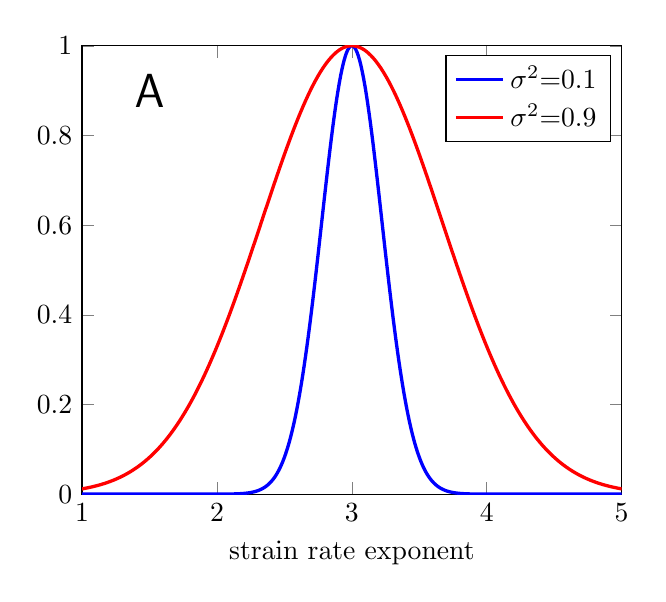
\begin{tikzpicture} 
\begin{axis}[ xlabel=strain rate exponent,xmin=1.0, xmax=5.0, ymin =0, ymax = 1.0 ] % invoke external gnuplot as % calculator: 
  \addplot [mark=none,very thick, blue, samples=1000]{exp(-(x-3.0)^2/0.1)}; 
  \addlegendentry{$\sigma^2$=0.1}
  \addplot [mark=none,very thick, red, samples=1000]{exp(-(x-3.0)^2/0.9)}; 
  \addlegendentry{$\sigma^2$=0.9}
\node[font=\fontsize{18}{18}\sffamily] at (axis cs:1.5,0.9){A};


\end{axis} 
\end{tikzpicture}
}
\hspace{-0.2cm}\subfigure{

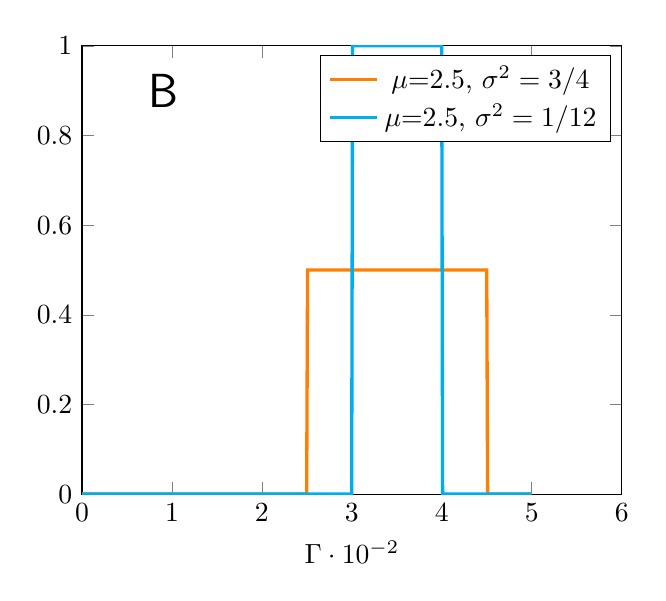
\begin{tikzpicture}[
    declare function={unipdf(\x,\xl,\xu)= (\x>\xl)*(\x<\xu)*1/(\xu-\xl);}
]
\begin{axis}[xlabel = $\Gamma \cdot 10^{-2}$,
    samples=1000,
%    const plot mark mid,
    xmin = 0, xmax = 6,
    ymin=0,ymax=1
]
\addplot [very thick, orange] {unipdf(x,2.5,4.5)};
 \addlegendentry{$\mu$=2.5, $\sigma^2 = 3/4$}
\addplot [very thick, cyan] {unipdf(x,3,4)};
 \addlegendentry{$\mu$=2.5,  $\sigma^2 = 1/12$}
\node[font=\fontsize{18}{18}\sffamily] at (axis cs:0.9,0.9){B};
\end{axis}
\end{tikzpicture}

}

\caption{(A) Normal distributions for the strain rate exponent prior (B) Uniform distributions for the strain rate exponent prior. In (A) we compare the possibility of using two different normal distributions to demonstrate our knowledge or lack thereof of what the values of the strain rate exponent should be. }
\label{fig:prior_ex} 
\end{figure}

 Another possibility is to use a \textit{non-informative prior} \citep{Tarantola05}. A non-informative prior gives equal likelihood (equal probability) to each value such that no preference is given to a single value. Using non-informative priors can be advantageous when it is not apparent what an acceptable value is, such as the strength of a weak factor An example of a non-informative prior is a uniform distribution for the strain rate exponent (Fig.\ref{fig:prior_ex}b). A uniform distribution has the following properties,
 \begin{align}
\mathcal{U}(a,b) =
\begin{cases}
 \frac{1}{b-a}   &b\geq x \geq a \\
               0 &\quad \text{otherwise} \\
\end{cases}
\end{align}
with a mean and variance of 
\begin{align}
\begin{split}
\mu(a,b) &=\frac{1}{2}(a+b) \\
\sigma^2(a,b) &=\frac{1}{12}(b-a)^2 .\ \\
\end{split}
\end{align}
The uniform distributions (Fig.~\ref{fig:prior_ex}b) have the same mean, but different variance. Compared to a normal distribution, the variance for the uniform distribution is determined by the range of likely values, each of which has the same probability.
	
 For a prior described by a normal distribution, a mean, $\mu$, and covariance, $\mathcal{C}$, are needed
\begin{equation}
\ppi_{prior} = \mathcal{N}(\mu,\mathcal{C})
\end{equation}
The negative log of the prior distribution results in a weighted misfit, or
\begin{equation}
\mathcal{J}_{prior} = \frac{1}{2}(\mm-\mm_{mean})^T\mathcal{C}^{-1}(\mm-\mm_{mean})
\end{equation}
With the prior, the cost function would be
\begin{equation}
\begin{split}
  \mathcal{J}(\uu,\mm,p)&:= \frac{1}{2}\int_{\partial \Omega_1} (\mathcal{O}\uu-\uu_{\text{obs}})^T\mathcal{C}^{-1}_{vel}(\mathcal{O}\uu-\uu_{\text{obs}})d\partial\Omega_1 \\
%  &+\frac{1}{2}(\eta_0 - \text{exp}({\int_{\Omega_i} \ln \eta}))^{2} \\
   &+(\eta_0 - \text{exp}({\int_{\Omega_i} \ln \eta}))^{2} +\frac{1}{2}(\mm-\mm_{mean})^T\mathcal{C}^{-1}(\mm-\mm_{mean}).
\end{split}
\end{equation}
While the solution to the adjoint equation does not change, the gradient term for each parameter becomes
\begin{equation}
\mathcal G:= \int_{\Omega} 2 \eta_{,i}(\IIinv, \Gamma, n, \sigma_y)\strain(\uu):\strain(\vv) d\Omega  + \mathcal{C}^{-1}(\mm-\mm_{mean})\mm_i.\
\end{equation}
These new gradients will be used to update the parameters as they measure the sensitivity of a parameter to an observation.


\section{Model Setup}
We have constructed a set of model constraints based on global observations with four components: A global temperature distribution, the geometry of faults, the kinematics of plate motion, and the geometry and bounds on the effective viscosity within selected regions.

The temperature model has been constructed globally in a spherical shell from which selected cross-sections are taken. The temperature of oceanic lithosphere follows a half-space cooling model using  updates to the digital grid of the age of the oceanic plates \citep{muller1997digital}.  
A thermal age was used within continental regions with the following three regions: Cratons (300 Ma), areas near subduction zones (75 Ma), and other areas (200 Ma), as detailed in \citep{Stadler27082010}.
The thermal structure of slabs were constructed as follows. 
Initially the top surface of the slabs was derived from the Slabs 1.0 surface, based on detailed seismic constraints, including seismicity and seismic reflection profiles \citep{Hayes2012}.
With normals pointing downward from this surface, an initial thermal structure of slabs based on the half space model using the age of the plate at the position of the trench was generated. This proceedure ensured continuity with the thermal structure of the oceanic lithosphere. Then, thermal conduction was solved for at each depth over a duration equal to the travel time to reach the depth with the local convergence velocity (using the relative velocity vector). Although solved only with conduction, this procedure resulted in thermal structures close to those obtained in fully dynamic models. The tops of thermal  slabs were sharp in the corner of the mantle wedge and then progressively became more diffusive with depth.
Within the lower mantle the thermal structure was based on scaled tomographic models,
including a P-wave\citep{simmons2012llnl} and a S-wave model \citep{ritsema1999complex}.
The lithosphere and upper mantle models and the upper and lower mantle were blended together at 75 km and 550 km depths, respectively, as shown in cross sections (Fig.\ref{fig:xsection2sumatra}).
We have used the seismo-tectonic approach for the shallower mantle and tomographic approach for the deeper mantle, as the seismic tomography models for slabs tend to be noisy.


On the surface of the earth we generated a veloctiy field from MORVEL56 \citep{GGGE2060} in a no net rotation (NNR) reference frame. Each cross-sectional model generally defines a great circle arc, with local unit vector \textbf{d} in the direction of the circle, such that we extracted the velocity $v_{xs}=\textbf{d}\cdot\textbf{v}$.  The NNR reference frame was used as the side-walls on the two-dimensional cross sections preclude any large-scale differential motion between the bulk of the mantle and the plates.

\begin{figure}[hbtp]
\centering
\scalebox{0.9}{
\hspace{-1.8cm}\subfigure[]{
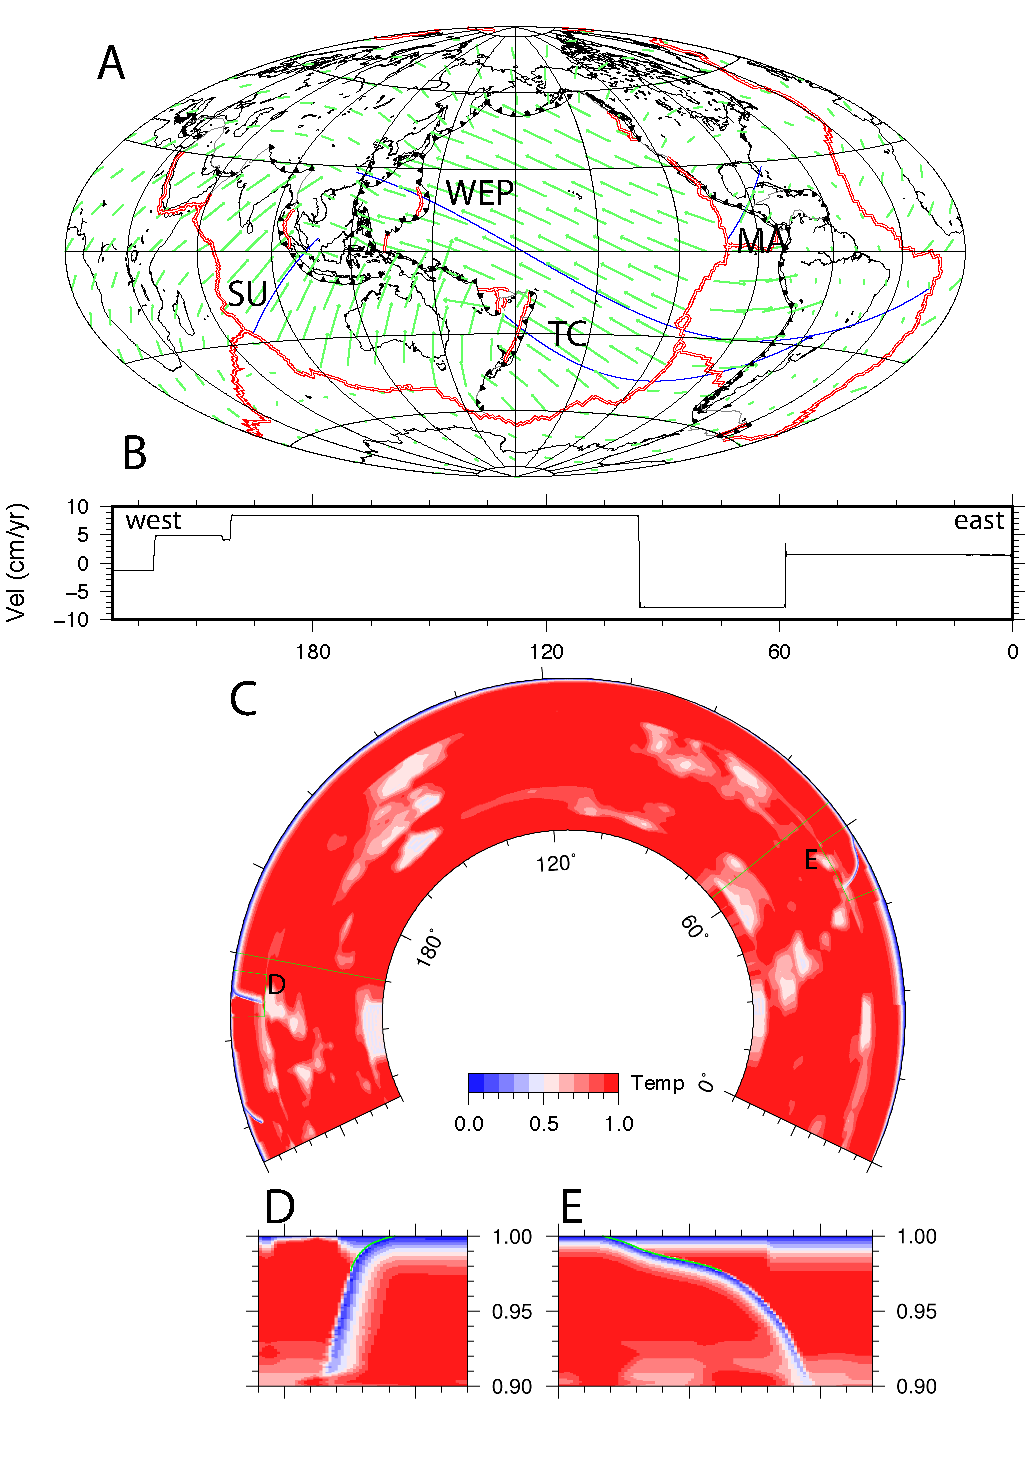
\includegraphics[height=150mm,width=100mm]{Summary_sections.pdf}%{mesh.pdf}
}

}
\caption{A. Velocity vectors in the no net rotation reference frame. Cross sections indicated with black lines, including western to eastern Pacific (WEP), Sumatra (SU), Tonga to Chile (TC) and Middle America (MA) B. Velocity in the direction of cross-section WEP.(C)Temperature distribution for cross section WEP. Zoom in of the Marianas (in D) and the Chilean (in E) slabs for the WEP cross section. In D and E, the solid green lines show the position of the weak zones.}
\label{fig:xsection2sumatra}
\end{figure}

Selecting a set of representative cross-sections in which all of the driving forces may be partially represented two-dimensionally is difficult, as it is likely that no plate and subduction zone is truly two-dimensional. 
Nevertheless, we have chosen a set of cross-sections in which plate motion was generally orthogonally to the strike of the trench and which represent some of the end-member cases from the least to the most seismically coupled subduction zones (Fig.\ref{fig:xsection2sumatra}A). To investigate the coupling for various seismically coupled subduction zones, we consider the cross-sections in Fig. \ref{fig:xsection2sumatra}. 
Our primary cross-section has the largest dimension (about $240^{\circ}$) and contains three subduction zones that span the range from the seismically coupled (Chile) to the least coupled (Marianas). This cross section contains one subduction zone with back-arc extension. The cross-sections in Fig.\ref{fig:xsection2sumatra}B, C are smaller than in  Fig.\ref{fig:xsection2sumatra}A, and thus do not contain the coupling variability of the larger cross-section; however those cross-sections represent other subduction zones that exhibit substantial coupling (Sumatra) and very little coupling (Tonga).




The fault zone decoupling between converging plates at subduction zones, generally thought to be the places on which great earthquakes occur, were represented as weak zones with unknown viscosity. 
A weak zone factor, created by a stencil with a center line defined by the Slabs 1.0 surface \citep{Hayes2012}, was defined as
\begin{equation}
\Gamma_{stencil} = 1.0 - (1-\Gamma_i)\exp\{-(d_i-d_0)^2/(2\cdot w^2)\}
\end{equation}
and with a coefficient $\Gamma_i$ that was recovered in ~\eqref{eq:rheo}, $d_0$ is the center-line profile, $w$ is the amount of smoothing for the weak zone.
 For our models, we assume the values of mantle parameters summarized in Table ~\ref{table:parameters}.

\begin{table}[H]
  \caption{Assumed parameters left as constants in the }
  \centering  % used for centering table
  \begin{tabular}{c c c} % centered columns (2 columns)
    \hline \hline                        %inserts double horizontal lines
    Symbol & Parameter & Value  \\ [0.5ex] % inserts table
    %heading
    \hline                  % inserts single horizontal line
    $\rho$ & Density ($\rho$)  & 3300 kg/m$^3$ \\
    $g$ & Gravity ($g$) & 9.81 m/s$^2$ \\
    $\alpha$ & Coefficient of Thermal expansion ($\alpha$) & 2 $\times$ $10^{-5}$ \\ 
    $\Delta T$& Temperature Difference $\Delta T$ & 1400 K \\
    $D$& Depth of layer ($D$) & 1500 km \\
    $\kappa$& Thermal Diffusivity ($\kappa$) & $10^{-6}$  m$^2$/s \\
    $\eta_{\text{ref}}$& Reference Viscosity  ($\eta_{\text{ref}}$) & $10^{20}$ Pa $\cdot$ s \\
    Ra & Rayleigh Number (Ra) & 2.92 $\times$ $10^9$ \\
    $n$ & Strain rate exponent in lower mantle ($n$) & 1.0 \\
    \hline %inserts single line
  \end{tabular}
  \label{table:parameters} % is used to refer this table in the text
\end{table}

\mgnote{\P~needs to be moved to the Discussion since in the end you do not factor in the uncertainty of your data. Move this \P, and then finish it with a discussion of how your method can be expanded.} A caveat in these cross-section optimizations is that both the tomography model and plate motion data are not unique and therefore have implicit uncertainty embedded within. For example, there are multiple tomography models that can be used in the lower mantle, such as the shear-wave model S40RTs \citep{ritsema2011s40rts} or the P-wave model (LLNL-G3Dv3) \citep{simmons2012llnl}), while plate motion data is dependent on the reference frame used such as plate motions with respect to hotspots, with respect to a specific plate (Pacific for example), or the no-net-rotation(NNR) reference frame. 
In addition to the uncertainty of the reference frame, there is uncertainty in the motion of one plate with respet to others which can possibly influence the parameter estimation of plate couplings. Therefore, while it is possible that the magnitudes of the rheological parameters may be different for different tomography and plate motion models, the overall relative (mechanical) coupling of subduction zones should not vary from those obtained from seismic coupling (\citep{scholz2012seismic}).


\mgnote{This is vague. The viscosity constraints need to be described in precise terms (e.g. magnetide of visocisty and geometry with reference citations}As presented earlier, the average effective viscosity data is an additional constraint that we will explore to determine the effect it has on the inference of the the rheological parameters. Since the effective viscosity is a constraint on the mantle from observations, then this data should better constraint on the global parameters such as the strain rate exponent, activation energy, and upper mantle prefactors. We will place the average effective viscosity constraint of $\overline{\eta}_i = 10^{19} Pa\cdot s$ under the South American plate \mgnote{Why note $10^21$ Pa-s? We can discuss}, (as it is the only plate in our models with a substantial continental plate overriding a subduction zone), as well as underneath Japan with $\overline{\eta}_i = 10^{19} Pa\cdot s$ \citep{hu2016asthenosphere} \vrnote{i need to find the exact dimensions used}.\mgnote{The specific outlines of the constrain on the viscosity}
 While we are able to solve this nonlinear Stokes flow, we need to resolve the thermal boundary layers and fault zones. Doing so requires either using very small elements with uniform refinement, which is not tenable as the forward problem would be computationally expensive. Therefore, we use adaptive mesh refinement (AMR) and refine in areas such as cold thermal boundary layers (oceanic plates) and fault zones (2 km resolution). 
We solve the nonlinear incompressible Stokes by linearizing the momentum equations, enabling the use of Newton's method \citep{rudi2015extreme}. 

\section{Results}

\mgnote{I haven't yet deleted the next not I made earlier as I think that the Results section still needs a lot of work. In the UQ subsection there are parts where you are starting to give this physical understanding of the results, when it comes to the conditiondistributions.}

\mgnote{Both of these sub-sections suffer from the same problem. You say we tried case x and we get y, but there is essentially no discussion of the 'why'. This is geodynamics, we are in the business of providing answers on the 'why'. How can you arrive at these concluions and discussions. You need to look at the equations, both of motion and  vicosity, perhaps plost of effective viscosity and then your condition distrbutions. I will give a lot of commentary in the days ahead on improving in this regard. Getting plots to use on Effective Vistory in cross sections would be really helpful.}

\subsection{Inversions}

From optimizations we infer plate coupling across subduction zones and global rheological parameters such as the yield stress and strain rate exponent globally for each cross-sectional model. Compared to our earlier studies \citep{ratnaswamy2015adjoint} where we knew what the actual values of the inferred parameters, these inversions we do not know what the true values are. Therefore, we test run a suite of tests to test both the initial guess and how well the data is constrained from the inversions by varying the initial guess of the strain rate exponent in Table \ref{table:initial_guess}. We vary the initial guess of the strain rate exponent from 2.0 to 3.5 as that range represents a lesser effect to a more pronounced effect of shear thinning in the upper mantle. From the recovered plate plate couplings and yield stress in Table \ref{table:initial_guess}, we are able to infer the same plate couplings and yield stress, independent of the initial guess which suggests that we avoid in local minimum for the inferred parameters. The independence of the initial guess also suggests that there is a stability in the inversions such that starting far away from the \textbf{MAP} point will lead to the same set of inferences.


After confirming the independence of the initial guess, we turn our attention to what the inferred values for the plate couplings as well as the global rheological parameters. We explore these parameter spaces because we not only want to understand what the values of the rheological parameters are, but if they fall within the bounds proposed by experimental studies. Therefore we infer the plate couplings and global rheological parameters such as the yield stress and strain rate exponent in Case 1, akin to what was done in \citep{ratnaswamy2015adjoint}.  In all models, we choose an initial weak zone factor of $\Gamma=10^{-5}$, which typically decouples the plate boundaries allowing subduction, an initial guess of 125 MPa for the yield stress because it provides a reasonable amount of dynamic weakening in forward models while satisfying estimates from seismicity \citep{craig2014reassessment}, while using an initial strain rate exponent of $n=3.0$, a value typically associated with mantle convection and within the bounds imposed from laboratory experiments \citep{ranalli1995rheology}, an activation energy $E_a=203.6$kJ/mol, a value we found through multiple forward models in which plates are sufficiently strong to act as stress guides. 


\begin{sidewaystable}

\centering

	\begin{table}[H]
		\caption{Case study summary\mgnote{ADD Footnote "Bold values are held fixed during the optimization"; "WEP: Western to eastern Pacific"}} % title of Table
		\centering  % used for centering table
		\begin{tabular}{c c c c c c c c  } % centered columns (2 columns)
		\hline \hline                        %inserts double horizontal lines
		Case & Subduction Zone & \textit{n} &$\sigma_y$&$\Gamma$ (SAM/RYU/IZU) $\cdot 10^{-5}$ &UM Prefactor &$E_a (kJ/mol)$&Visc. data   \\ [0.5ex] % inserts table
		%heading
		\hline                  % inserts single horizontal line
          1 &WEP& 3.046 & 146 & $67.3/0.773/0.798$ & \textbf{2000} & \textbf{203.5} & no \\
	      	 2 &WEP& 3.042 & 148 & $100/0.82/0.77$ &  4922.3& \textbf{203.5} & no  \\
	        3 &WEP& 3.08 & 141.8 & $87.3/0.703/0.7448$ & \textbf{2000} & \textbf{203.5} & yes \\
	        4 &WEP& 3.0225 & 155 & $94.6/0.8423/0.889$ & \textbf{2000} & \textbf{203.5}& priors used \\
             5 &WEP& 3.072 & 147.2 & $85.1/0.702/0.814$ & \textbf{2000} & 219.7& priors used \\
             6 &WEP& 3.061 & 137.9 & $73.6/0.754/0.792$ & \textbf{2000} & 219.7& priors used and visc. data \\
             7 &WEP& 3.061 & 137.9 & $73.6/0.754/0.792$ & \textbf{2000} & 219.7& priors used and visc. data \\

                7 &Sumatra& 3.048 & 143.1 & $63.9$ &  \textbf{2000}& \textbf{203.5}& no \\

                 8 &Sumatra& 3.1 & \textbf{120} & 44.1 & \textbf{2000} & 207.2   &no\\
                  9 &Sumatra& \textbf{3.0} & 128.1 & 38.2 & \textbf{2000} & 190.7   &no\\
              10 &Tonga  & 3.0621 & 139.1 & 2.21& \textbf{2000} & \textbf{203.5} &no  \\              
               11 &Tonga  & 3.051 & 135.2 & 0.7& \textbf{2000} & 186.2 &no  \\             
              12 &Tonga  & 3.087 &  \textbf{120} & 0.71 &\textbf{2000} &175.6  &no  \\              
               13 &Tonga  & \textbf{3.0}  & 127.7 & 0.8 &\textbf{2000} &198  &no  \\             
               14 &Central America  & 3.0621 & 139.1 & 2.21& \textbf{2000} & \textbf{203.5} &no  \\           
                 15 &Central America  & 3.12 & \textbf{120} & 6.3& \textbf{2000} & 178.1 &no  \\       
                 16 &Central America  & \textbf{3.0} & 132.1 & 0.84& \textbf{2000}& 207.2 &no  \\        
          
          
                \hline %inserts single line
		\end{tabular}
		\label{table:inversions} % is used to refer this table in the text
		\end{table}
\end{sidewaystable}



\mgnote{The problem with the organization is that you have just described how you will demsonstrate how the inversions worka and what they depend on. But instead, you launch into you keep finishing this ordering of plate coupling. The later is fundamental, but you need to stick to your organization.} 
In Case 1 for the WEP cross-section, we find that even though we used the same initial guess for the weakfactors, we find that the recovered values are different, with the South America subduction zone having the largest plate coupling. Furthermore, the inferred strain rate exponent suggest that there is significant amount of shear thinnning in thee upper mantle. While the plate couplings, yield stress and strain rate exponent are important parameters to infer, a natural question to ask would be how would these parameters change if another global parameter would be included such as the upper mantle prefactor. Therefore, we infer the plate couplings, yield stress, strain rate exponent and upper mantle prefactor in Case 2. We find that the inferred couplings are different than those from Case 1 in Table \ref{table:inversions}, while the strain rate exponent is similar to what was inferred in Case 1 ($0.113\%$) as well as the yield stress in Case 2 ($1.37\%$).  

An important parameter that we did not previously explore in \citep{ratnaswamy2015adjoint} was the activation energy, which controls the amount of viscosity dependence based on the temperature. Inferring the activation energy would help place bounds on how strong slabs are and to what degree the weakening in the upper mantle is due to the activation energy. In Case 3, we find that the inferred activation energy is 
$212.8 kJ/mol$, while finding an increase in the strain rate exponent. Furthermore, we find that the yield stress is larger than the values inferred in Cases 1-2, while the upper mantle prefactor is larger than  what was inferred in Case 2. An important part of our inversions is to impart knowledge in the form of priors to reduce the amount of uncertainty of the inferrred parameters.

Using prior distributions, we repeat Cases 1-4 for WEP in the subsequent Cases 5-8.  For the plate couplings we use a normal distribution with a mean of $10^{-5}$ with a large variance so that the inferred parameters can be guided by the misfit from the cost function. We find in Case 5, that the inferred strain rate exponent is 3.062, which is similar to what was inferred in Cases 1-4. Furthermore, the inferred yield stress is 138 MPa, which suggests that there is less dynamic weakening than what was found in Cases 1-4. When we infer the strain rate exponent, we find that the inferred strain rate exponent is larger than the values inferred in Cases 1-4. Furthermore, we find that the amount of adjoint iterations for convergence is approximately 7-8, similar to what was found in Cases 1-4.

Similarly to the strain rate exponent, we find that the activation energy is approximately $5\%$ larger than what was inferred in Case 4. Instead of using prior distributions as knowledge, we will use average effective viscosity as a constraint in areas under continents and under Japan. Using this knowledge, we want to determine if we can refine our estimates of the inferred rheological parameters. Repeating Cases 1-4, we find in these cases that the inferred strain rate exponent are all greater than 3.05, while in Case 12, we find that the inferred activation energy is $222 kJ/mol$. An important point would be to combine both prior knowledge and the average effective viscosity data. 

Using both prior knowledge and average effective viscosity data, we again repeat Cases 1-4. Doing so, we  find that the inferred strain rate exponent is 3.07 in Case 16, which is less than $5\%$ from what was found in Case when using average effective viscosity data. Furthermore, we find that the inferred yield stress is approximately 139 for Case 17, while in Cases 18-24 the inferred yield stress is on average 143 MPa. While the inferred strain rate exponent and yield stress are not significantly changed, we must determine if the activation energy would be. Therefore, in Case 22, we find that the inferred activation energy is $229 kJ/mol$, which is $3.15 \%$ more than what was inferred in Case 12. 


A new parameter that is included in the inversion for Case 1 is the upper mantle prefactor, which plays an important part in controlling the effective viscosity (increasing this prefactor would increase the effective viscosity) and the amount of shear thinning in the upper mantle. We find that we are able to infer the upper mantle prefactor within 5 adjoint iterations, thus demonstrating that this parameter can be inferred within a reasonable amount of iterations.


	
While we explored the influence of the global parameters and plate couplings with the additional upper mantle prefactor parameter, it would important to see if there is any change to the ordering of the plate couplings by just inferring the yield stress and strain rate exponent with those couplings. We do so in Case 2 by  keeping the upper mantle prefactor fixed, effectively conditioning the upper mantle pre-factor (similarly done in \citep{ratnaswamy2015adjoint}). In this case, we find that the inferred strain rate exponent is 3.042, which is close to the initial guess of 3.0, (similar to Case 1) and is only $\approx$ 0.1\% larger than the inferred strain rate exponent in Case 1. Similar to the strain rate exponent, the inferred yield stress in Case 2 is 146 MPa, only $\approx$1\% lower than the inferred yield stress in Case 1, while the inferred plate couplings follow the same pattern as the least coupled subduction zones are Ryukyu and Izu-Bonin. We see in Fig.\ref{fig:inverse1}a, that we not only recover different plate couplings for the three subduction zones but that their relative ordering is the same as in Case 1, possibly suggesting that the physics of these mantle flow models prefer this relative plate coupling ordering. 

\begin{table}[H]
		\caption{Sensitivity of initial guesses for Case 1} % title of Table
		\centering  % used for centering table
		\begin{tabular}{ c c c c } % centered columns (2 columns)
		\hline \hline                        %inserts double horizontal lines
		 $n_{guess}$ &$n_{infer}$ &$\sigma_y$&$\Gamma $(SAM/RYU/IZU) $\cdot 10^{-5}$   \\ [0.5ex] % inserts table
		%heading
		\hline                  % inserts single horizontal line
        	 2.0 &3.042 & 146 & $99.2/0.81/0.772$   \\
	         2.95 &3.042 & 148 & $100/0.82/0.77$\mgnote{Is "100" a bound?}    \\
	         2.98 &3.046 & 146 & $67.3/0.773/0.798$  \\
	        3.5 &3.042 & 146.3 & $99.4/0.811/0.771$  \\             
                \hline %inserts single line
		\end{tabular}
		\label{table:initial_guess} % is used to refer this table in the text
		\end{table}



\mgnote{Specifically, is the effective viscosity before you add this additional constraint larger or smaller than the effective viscosity constraint? Look at this for both the whole upper mantle as well as in the specific area that the effective viscosity constraint is added.}

  % The first case study is shown below in Fig.\ref{fig:inverse1}
\begin{figure}[H]
\centering

\hspace{-0.2cm}\subfigure{
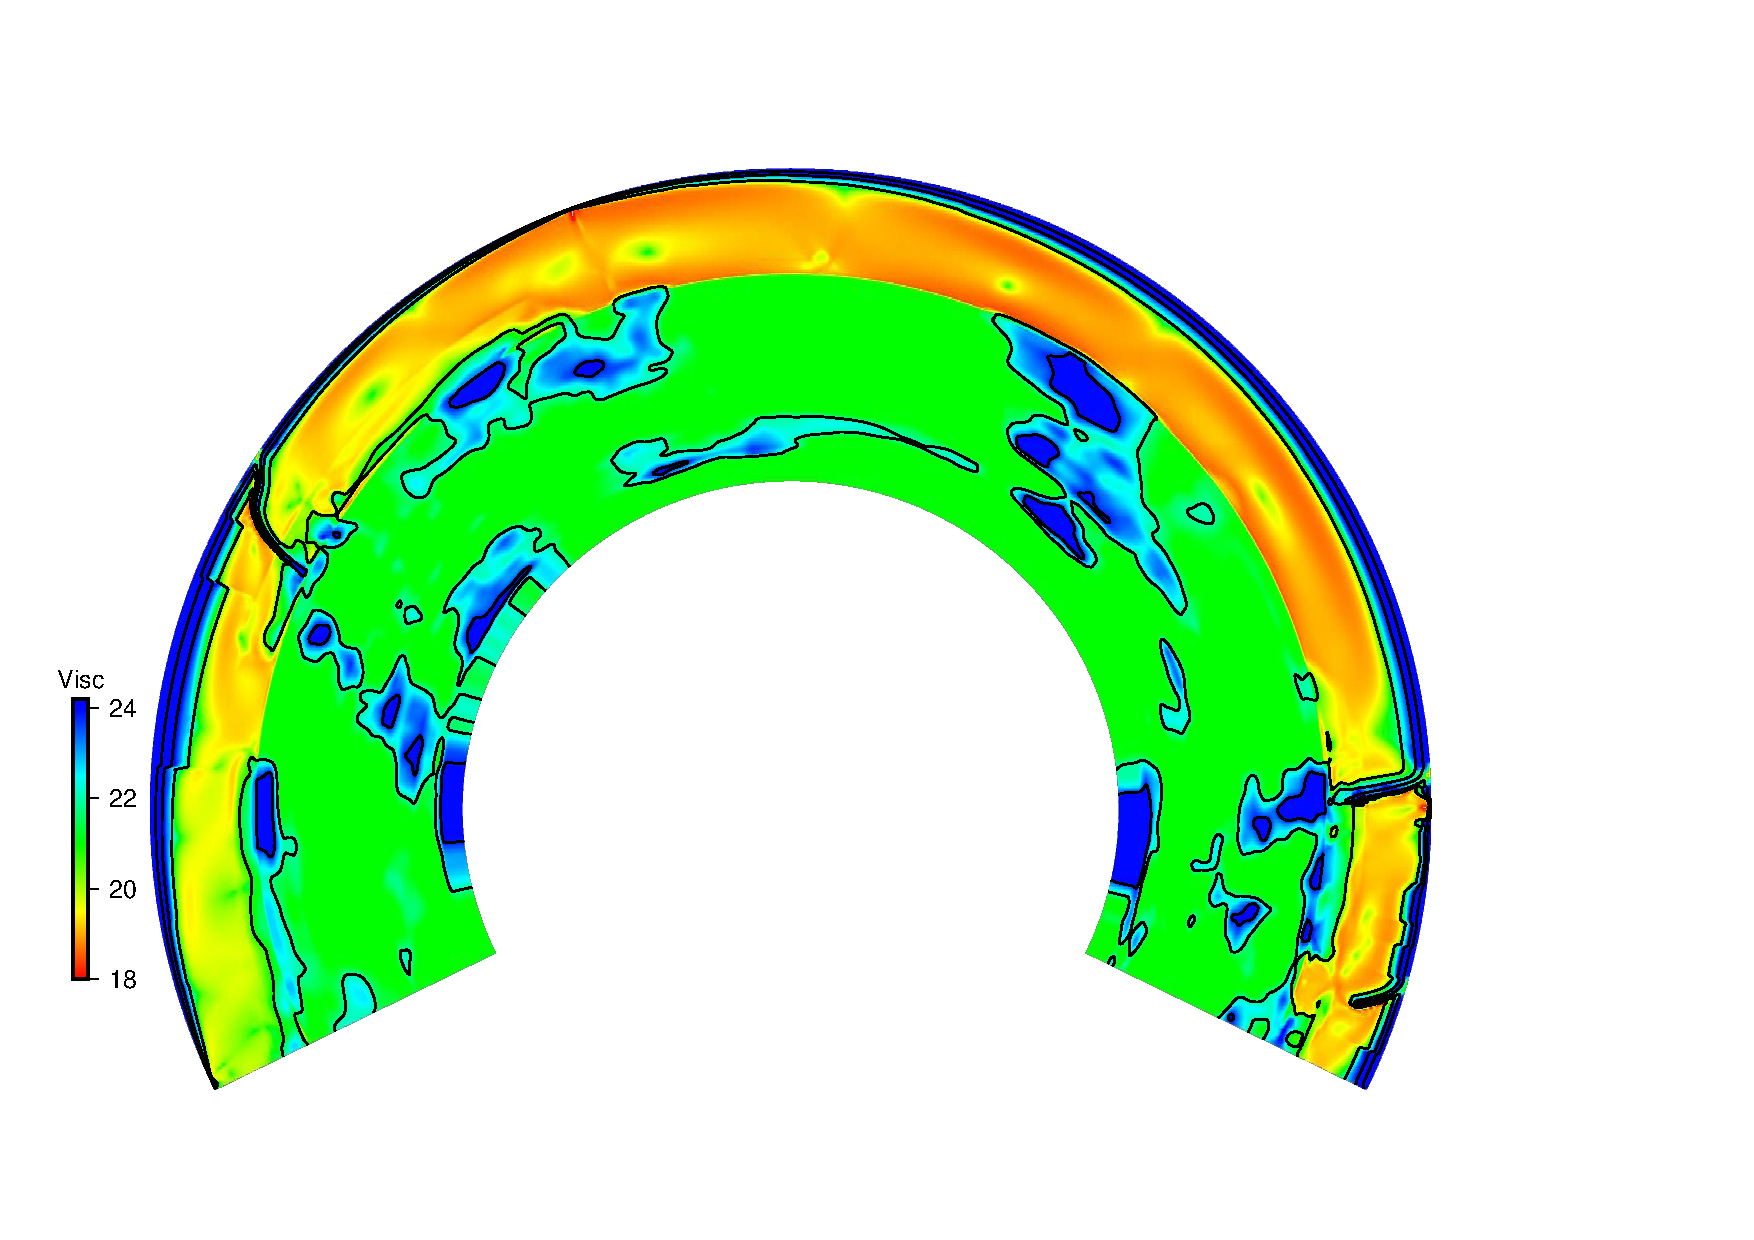
\includegraphics[height=65mm,width=128mm]{vish_contour.pdf}%{mesh.pdf}
}
\hspace{-0.4cm}\subfigure{
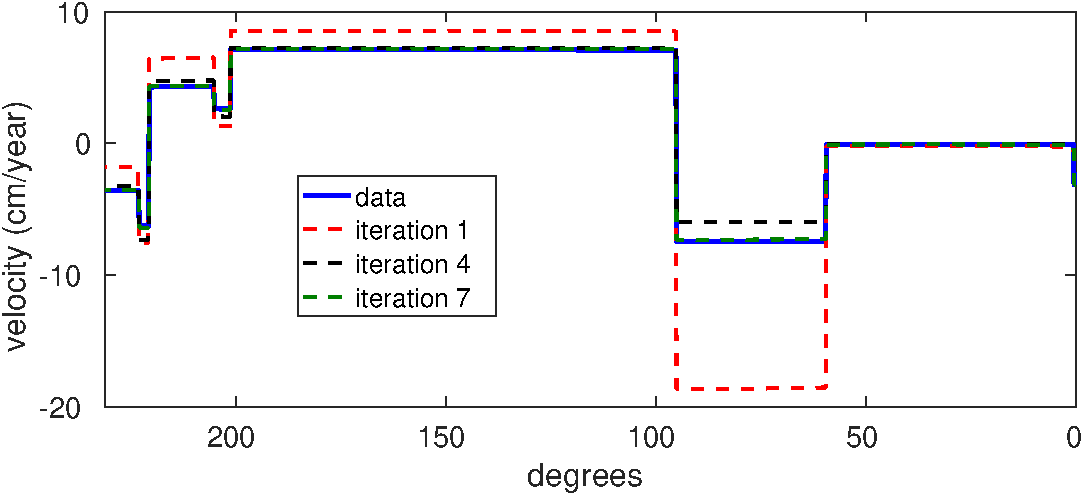
\includegraphics[height=35mm,width=58mm]{data_morvel.pdf}%{mesh.pdf}
}
\hspace{-0.2cm}\subfigure{
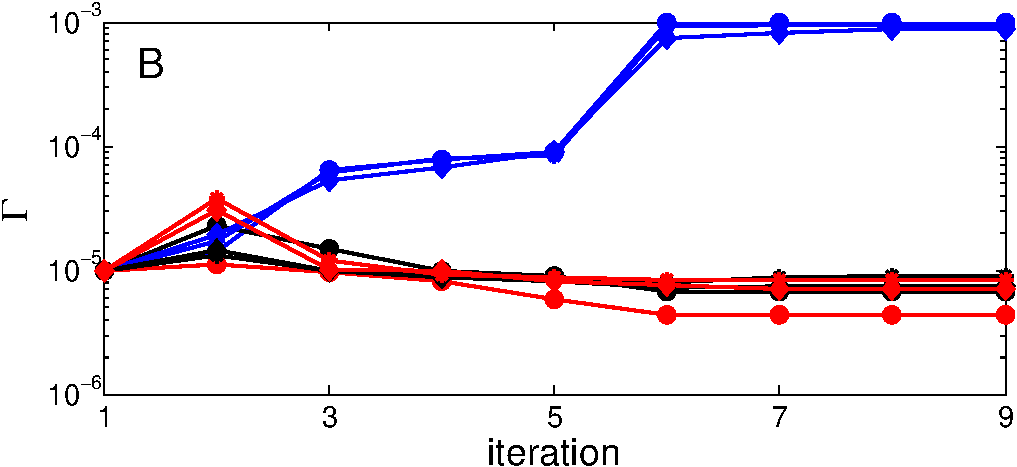
\includegraphics[height=35mm,width=58mm]{fig3b.pdf}%{mesh.pdf}
}
\hspace{-0.4cm}\subfigure{
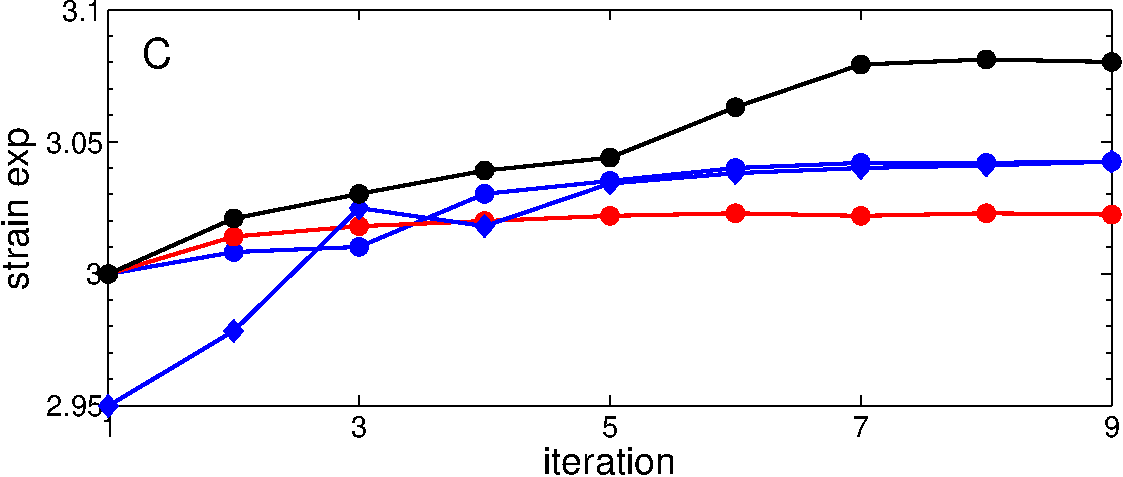
\includegraphics[height=35mm,width=58mm]{fig3c.pdf}%{mesh.pdf}
}
\hspace{-0.2cm}\subfigure{
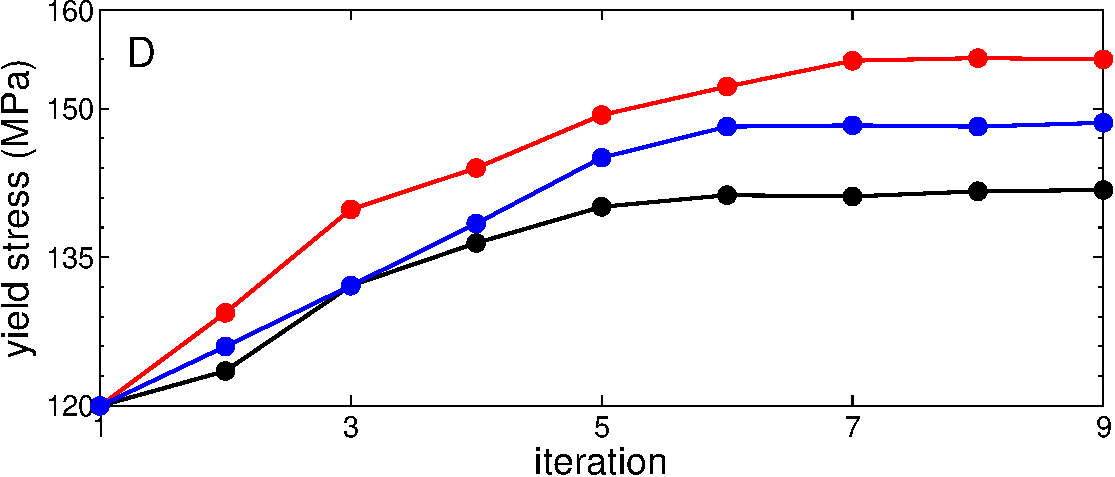
\includegraphics[height=35mm,width=58mm]{fig3d.pdf}%{mesh.pdf}
}
%\hspace{-0.2cm}\subfigure[]{
%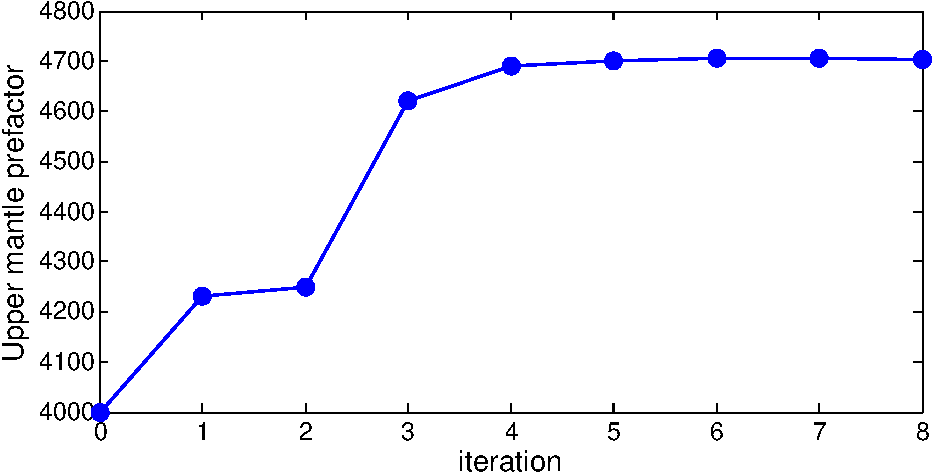
\includegraphics[height=35mm,width=58mm]{um_chap4.pdf}%{mesh.pdf}
%}

\caption{\mgnote{The labels in the Figure don't correspond with those in the Caption.}
(A) Effective viscosity for Case 1. \mgnote{Distance is flipped compared to Fig. 2C. Also the aspect ratio is messed upi -- it is stretched horizontally.}
(B) Surface velocity comparison between data and different iterations (Case 1). \mgnote{We need a zoom in on the velocity near the back-arc basin. This could be made a as an "insert". Please come by and see me for what I mean.}
(C) Plate boundary weakfactor iteration (South America (blue lines), Izu-Bonin (red lines), Ryukyu (black lines), with \textit{circles} being velocity data only, \textit{diamonds} \mgnote{Diamonds need to be made open diamonds because it is impossible to easily distinguish them from the close circles.} being velocity and effective viscosity data and \textit{asterisks} \mgnote{I can't see any asterisks} being velocity and priors  (d) strain rate exponent iteration \textit{blue circle} being plate velocities, \textit{blue diamonds} being a different initial guess, \textit{black circle} being velocity and effective viscosity data and \textit{red circle} being velocity and priors (e) yield stress iteration with \textit{blue circle} being plate velocities, \textit{black circle} being velocity and effective viscosity data and \textit{red circle} being velocity and priors .
\mgnote{Figure is too confusing. Symbols and colors need to be used in the same way in B-D. Please comeby and we can discuss why.}
}
\label{fig:inverse1}
\end{figure}

\mgnote{What about the convergence rate when priors are used? Describe.}
While using additional data may reduce the uncertainty of the inferred parameters, 
\mgnote{Is this a generic statement or something that you have just demonstrated?}
the inclusion of prior knowledge would certainly aid in reducing the variance of the inferred parameters. Using knowledge from experimental data \citep{korenaga2008new}, we include prior knowledge as Gaussian distributions with mean values of $\overline{n}=2.95$, $\overline{\sigma}_y = 120$ MPa, and $\overline{\Gamma}=10^{-5}$, while using variances that do not place strong constraints on the inferred parameters (Case 4). 


 % The first case study is shown below in Fig.\ref{fig:inverse1}
\begin{figure}[H]
\centering

\hspace{-1.0cm}\subfigure{
}

\hspace{0.2cm}\subfigure{
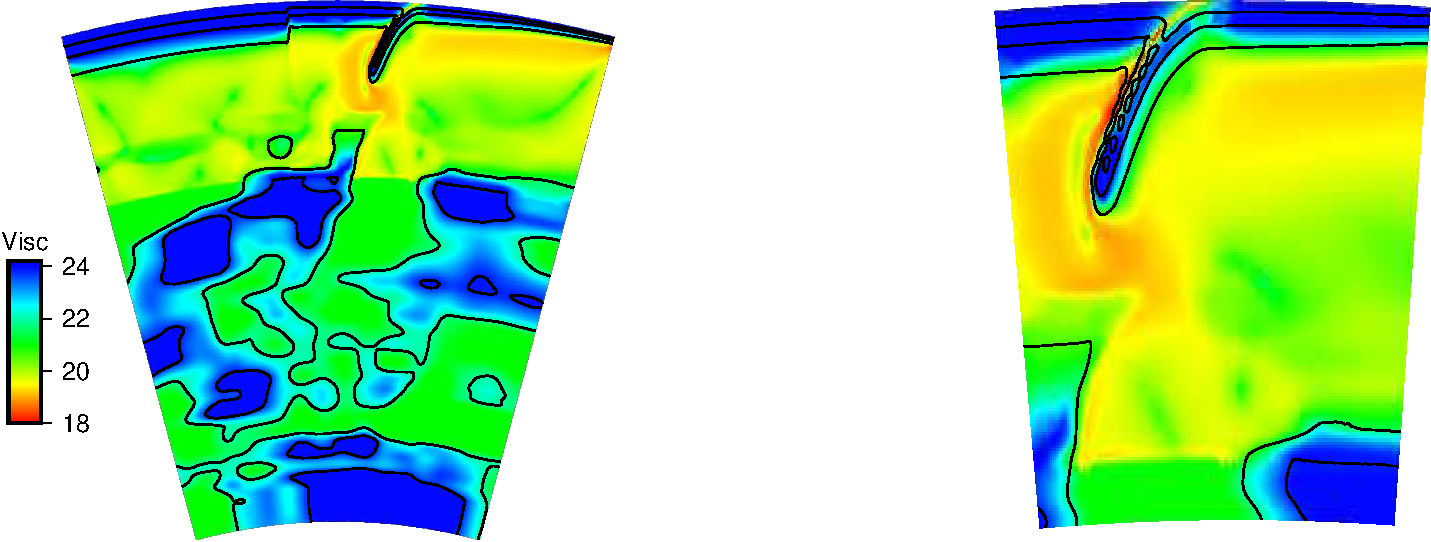
\includegraphics[scale=0.7]{middle.pdf}%{mesh.pdf}
}
%\hspace{-0.2cm}\subfigure[]{
%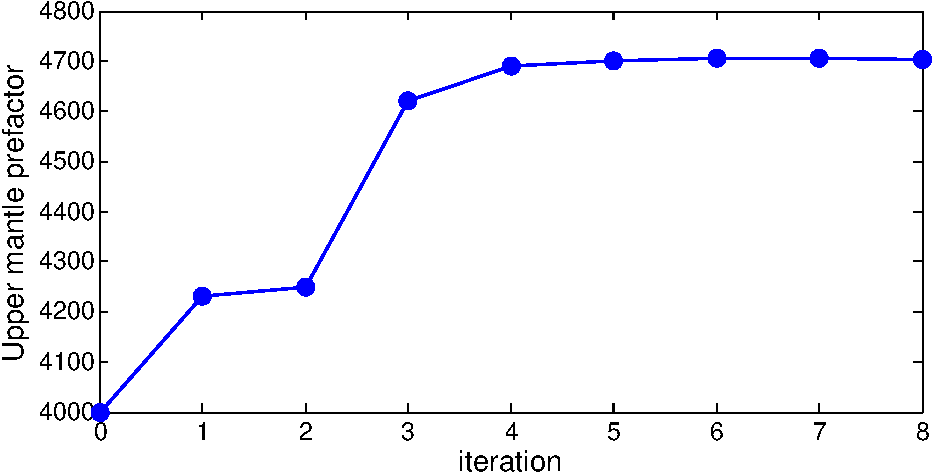
\includegraphics[height=35mm,width=58mm]{um_chap4.pdf}%{mesh.pdf}
%}
\caption{\mgnote{ Case number}
Effective viscosity for (A) Sumatra \mgnote{Need outline of zoom in areas in A and C.} (B) Zoom in of Sumatra subduction zone (C) Central America (B) Zoom in of Central America subduction zone.}
\label{fig:visc_smaller}
\end{figure}

While the larger cross-section (Cases 1-4) has the advantage of having subduction zones of varying seismogenic coupling, it is important to compare the parameter inferences from the larger cross-section (WEP) to other cross-sections with different subduction zones to determine if the global parameters would be of similar magnitude and how. 
The Sumatra subduction zone is of particular interest as it is thought to be one of the more seismically coupled subduction zones. Therefore, we repeat similar case studies as was done for WEP. For Sumatra, we find in Case 21, that the global strain rate exponent is 3.08, while 3.063 for when priors are imposed. When it comes to the activation energy, we find a value of $217.4 kJ/mol$ when we do not include prior knowledge, while 
with prior knowledge we find a value of $224.9 kJ/mol$. Furthermore, the inferred yield stress ranges from 132.6 MPa to 141.7 MPa, values that are similar to what were obtained in WEP. While the Sumatra model is a different subuction zone than was was examined in WEP, we find that there is a similar value for the plate coupling for Sumatra.
 % The first case study is shown below in Fig.\ref{fig:inverse1}
\begin{figure}[H]
\centering
%\hspace{-0.2cm}\subfigure[]{
%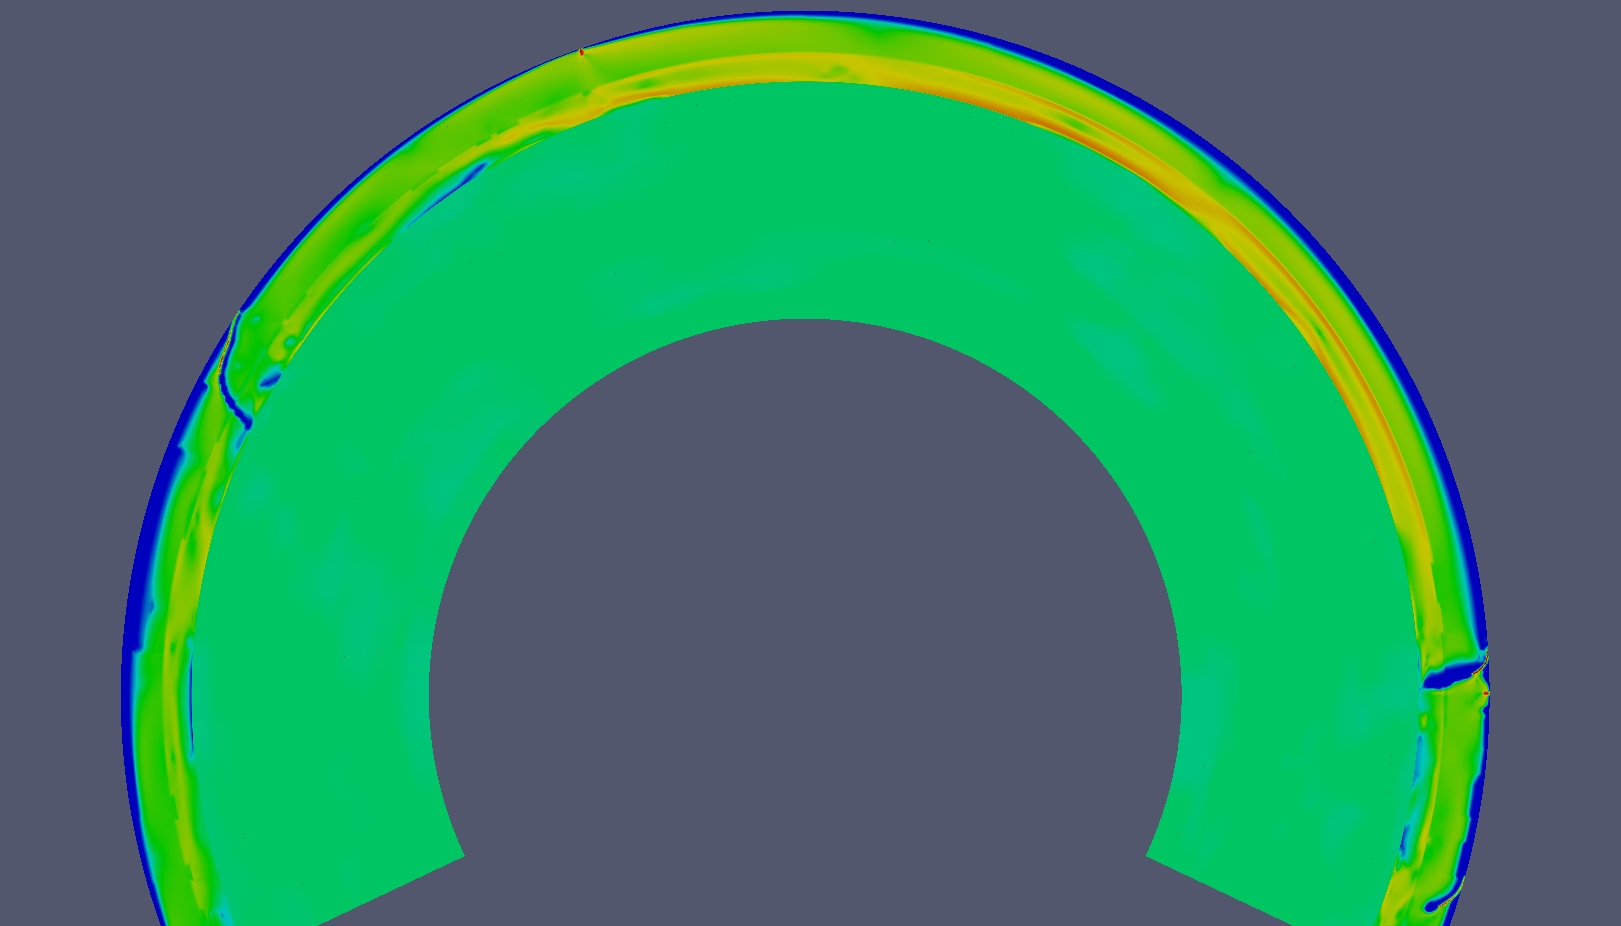
\includegraphics[height=65mm,width=128mm]{visc_no_stress.jpg}%{mesh.pdf}
%}
\hspace{-0.4cm}\subfigure{
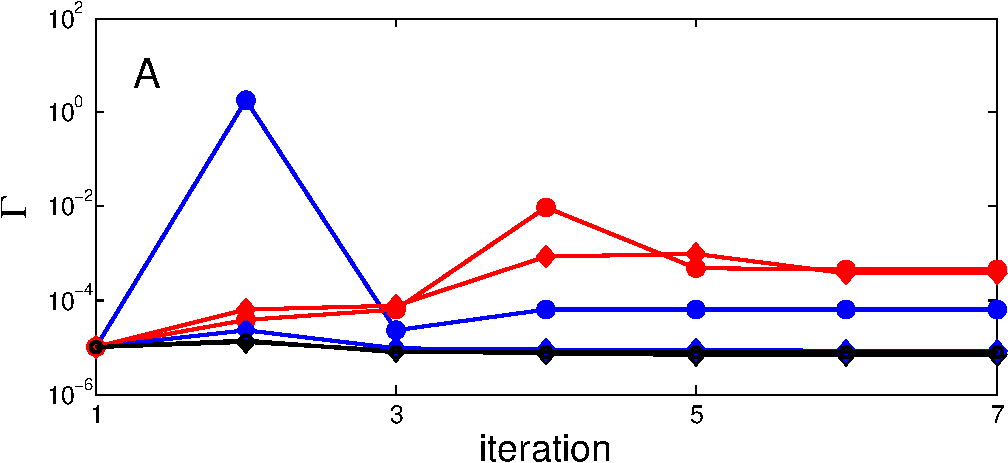
\includegraphics[height=35mm,width=58mm]{fig4a.pdf}%{mesh.pdf}
}
\hspace{-0.1cm}\subfigure{
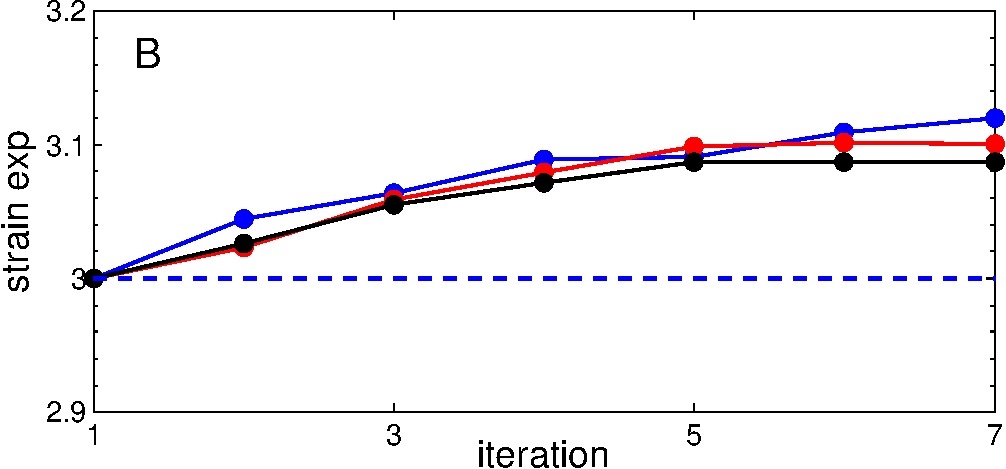
\includegraphics[height=35mm,width=58mm]{fig4b.pdf}%{mesh.pdf}
}
\hspace{-0.2cm}\subfigure{
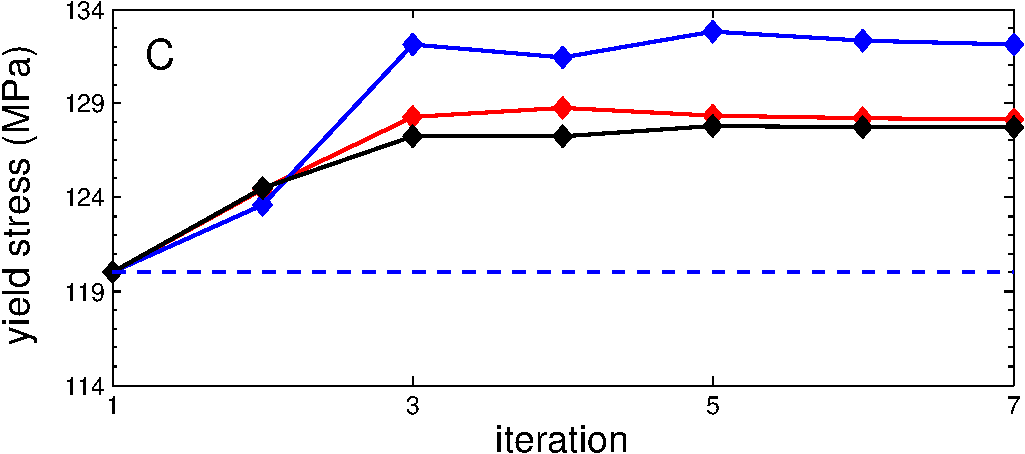
\includegraphics[height=35mm,width=58mm]{fig4c.pdf}%{mesh.pdf}
}
\hspace{-0.2cm}\subfigure{
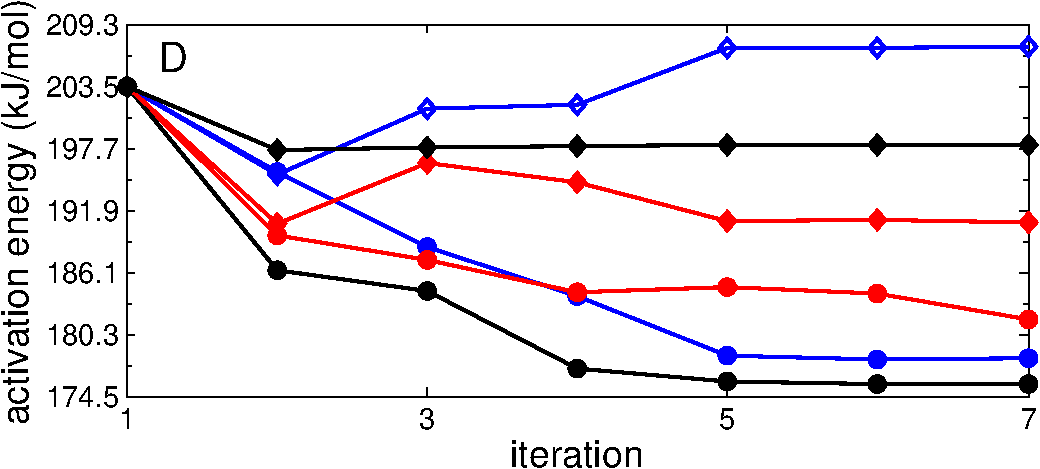
\includegraphics[height=35mm,width=58mm]{fig4d.pdf}%{mesh.pdf}
}
%\hspace{-0.2cm}\subfigure[]{
%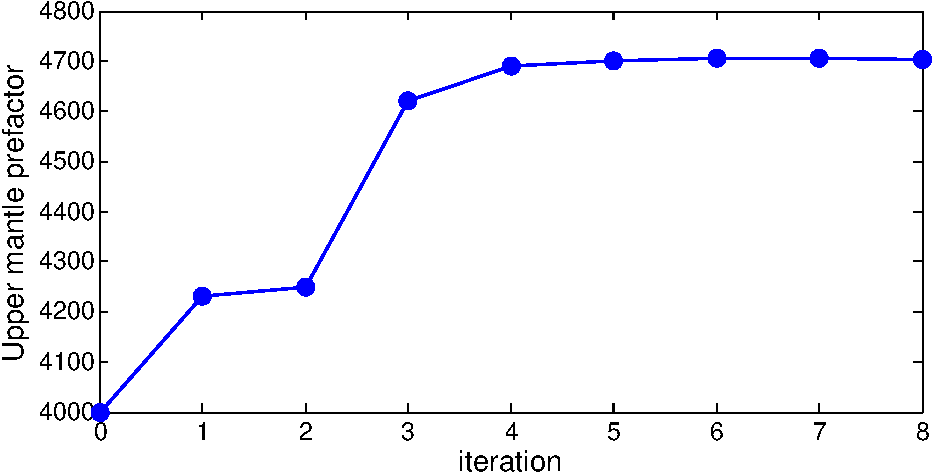
\includegraphics[height=35mm,width=58mm]{um_chap4.pdf}%{mesh.pdf}
%}
\caption{(A) Plate boundary weakfactor iteration for Central America (blue lines), Sumatra (red lines), Tonga (black lines). \textit{Diamonds} \mgnote{Need to use Open Diamond} represent inversion with strain rate exponent held fixed\mgnote{Case ?}, while \textit{circles} represent yield stress held fixed (C) strain rate exponent iteration, \textit{dashed line} represents the fixed value of yield stress (D) yield stress iteration \textit{dashed line} represents the fixed value of the strain rate exponent.
\mgnote{No cap for B? No dashed line in D.}}
\label{fig:inverse1}
\end{figure}
\mgnote{What is the objective here? This \P~ is confusuing because there is all this discussion about Sumatra, bute the WEP models are being referred to} We find in Case 5, that the inferred strain rate exponent is approximately 3.05, while the yield stress is approximately 143 MPa. The inferred plate coupling for Sumatra is larger than that of Ryukyu and Izu-Bonin in Cases 1-4, which seems to further suggest that mechanical coupling is independent of rheology. 

Central America is another cross-section that we consider as it has large magnitude events. We again repeat the same case studies that were done for Sumatra to ascertain the rheological parameters to see how much they vary between cross-sectional models. We find a similar value for the strain rate exponent as was found for WEP and Sumatra, with an inferred strain rate exponent of 3.062, where the largest value is 3.12 without using priors. When priors are used, the strain rate exponent is 3.051, which is similar to what was inferred in Case and for WEP and Sumatra respectively. A natural question to ask is whether the activation energy remains the same for Central America compared to WEP and Sumatra. We explore this in Cases 2 -9 and find that the inferred activation energy is approximately $245$ kJ/mol, while when priors are used the activation energy is approximately $229$ kJ/mol-both values being larger than what was inferred from WEP and Sumatra. 

The last cross-section we considered was Tonga as it represents one of the end-member cases with regards to seismic coupling. Therefore, determining whether the rheological parameters such as the strain rate exponent and activation energy would change would be an important result to determine. Similar to the previous three cross-sections, we infer a combination of plate coupling and the global rheological parameters to ascertain how coupled Tonga is relative to the other subduction zone models, and if there are any large changes to the inferred global parameters compared to the previous cross-section models. We find that the the inferred strain rate exponent is in the range of 3.07-3.11 for Cases -, where there inference is solely governed by the misfit in plate motions. The inferred yield stress from the inversions is approximately 146.2 MPa - 157.9 MPa, suggesting that there is less yielding in the hinge zones for the Tonga cross-section. With regards to the activation energy, we find that the inferred activation energy is between 226 - 249 kJ/mol. When we impose priors, we find that the inferred strain rate exponent is reduced now to 3.04-3.062, while the yield stress is reduced to the range of  131-140.2 MPa. A similar trend is noted for the activation energy where the inferred values with priors is in the rage of 217-226 kJ/mol.



While we are able to infer the global parameters and the activation energy, there is still is a question as to whether the plate coupling for Sumatra would change if we kept one of the global parameters fixed. To this end, we explored this question by fixing either the yield stress or strain rate exponent and inferring the plate coupling and activation energy in Cases 6-7. When the yield stress is fixed (Case 7), we find that there is a slight increase in the strain rate exponent, while the inferred plate coupling is still larger than Ryukyu and Izu-Bonin. Similarly, when the strain rate exponent is fixed (Case 8), the yield stress increases slightly from the initial guess, while the plate coupling for Sumatra is still larger compared to Izu-Bonin and Ryukyu. 








\subsection{Uncertainty Quantification for Plate boundary stresses}

An important part of our study is to quantify the uncertainty of the inferred rheological parameters by examining the posterior distributions, more specifically the conditional distributions. The conditional distributions convey not only the uncertainty in each parameter, but the trade-offs and how they contribute to the underlying physics of these models. In Fig.\ref{fig:distrib}a,b, we compare the conditional distributions for the plate couplings vs. yield stress and strain rate exponent in Case 1 and find that there is a clear demarcation between the least coupled subduction zones (Ryukyu and Izu-Bonin) and South America. The partitioning of the subduction zones suggest that the South America plate boundary is more mechanically coupled compared to Ryukyu and Izu-Bonin regardless of the global parameter (yield stress and strain rate exponent). Furthermore, we find a similar partitioning for Cases 2-3 for the larger cross-section, which seems to suggest that regardless of prior knowledge or average effective viscosity data being used in these inversions, there still is a preferential ordering with regards to plate coupling. 

An important consequence of these conditional distributions are the trade-offs between the rheological parameters. We are able to  We see that there exist strong positive correlations between the strain rate exponent and yield stress in Fig.~\ref{fig:distrib}c, a negative correlation between the plate couplings and yield stress in Fig.~\ref{fig:distrib}b and a slight positive correlation between plate couplings and strain rate exponent in Fig.~\ref{fig:distrib}a that were previously observed in \citep{ratnaswamy2015adjoint}. The positive correlation between the strain rate exponent and yield stress suggests that as the strain rate exponent increases, plate motions increase, thereby resulting in an increase in yield stress in order to compensate for the increase in plate velocity. 
Yield stress and strain-rate exponent both control the degree of nonlinearity of the system; nonlinearity is increased with a large $n$, so $\sigma_y$ must decrease in order to fit the kinematic constraints.
Likewise, the increase in plate coupling which reduces plate velocity causes an increase in viscosity.  To compensate for this increase in viscosity, a decrease in yield stress is needed, which causes weakening in plates, thereby increasing plate motion. Similarly, as plate coupling increases (increase in viscosity in the fault zone), an increase in the strain rate exponent is needed as compensate for the decrease in plate motion.  
%A new parameter that we included in our inferences is the upper mantle prefactor, a value that controls the effective viscosity in the upper (or lower) mantle. We find that there exists strong correlation between the upper mantle prefactor and strain rate exponent. This correlation is not surprising as the effective viscosity is highly dependent on the upper mantle prefactor and the strain rate exponent, i.e. an increase in strain rate exponent leads to more shear thinning (decrease in effective viscosity), which would give rise to an increase in the upper mantle prefactor.

\begin{figure}[H]
\centering
\hspace{-0.85cm}\subfigure[]{
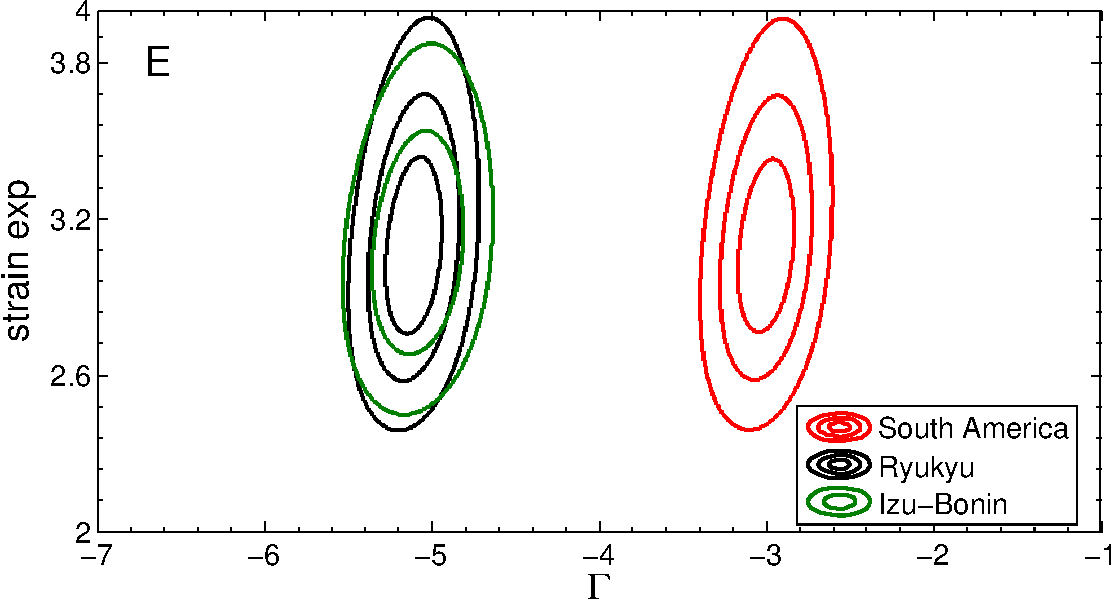
\includegraphics[height=35mm,width=52mm]{fig5a.pdf}%{mesh.pdf}
}
\hspace{-0.1cm}\subfigure[]{
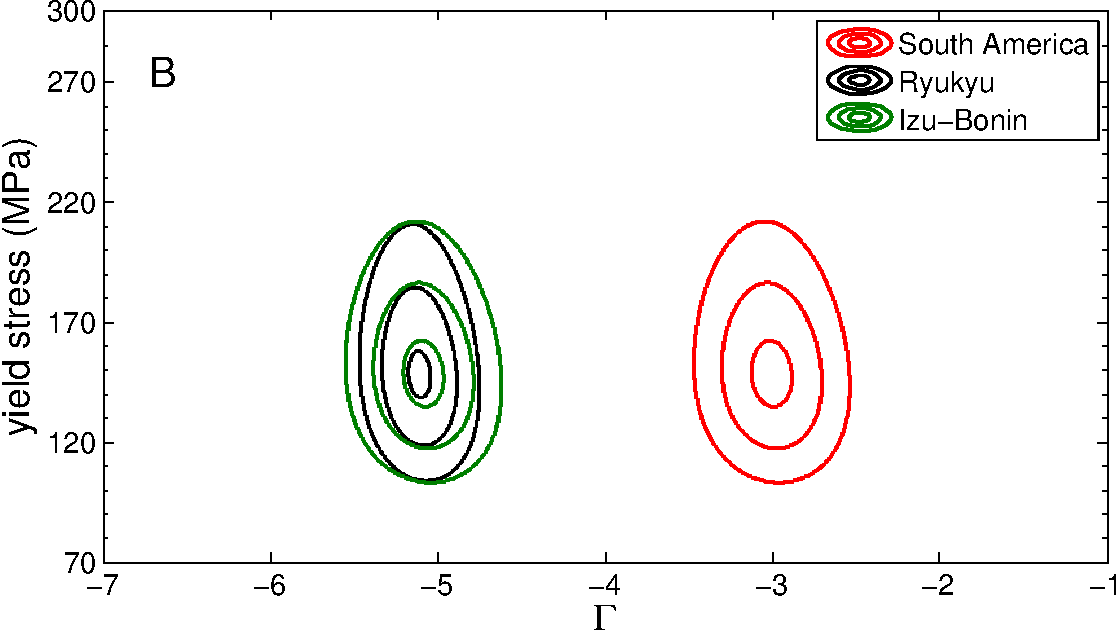
\includegraphics[height=35mm,width=52mm]{fig5b.pdf}%{mesh.pdf}
}
\hspace{-0.1cm}\subfigure[]{
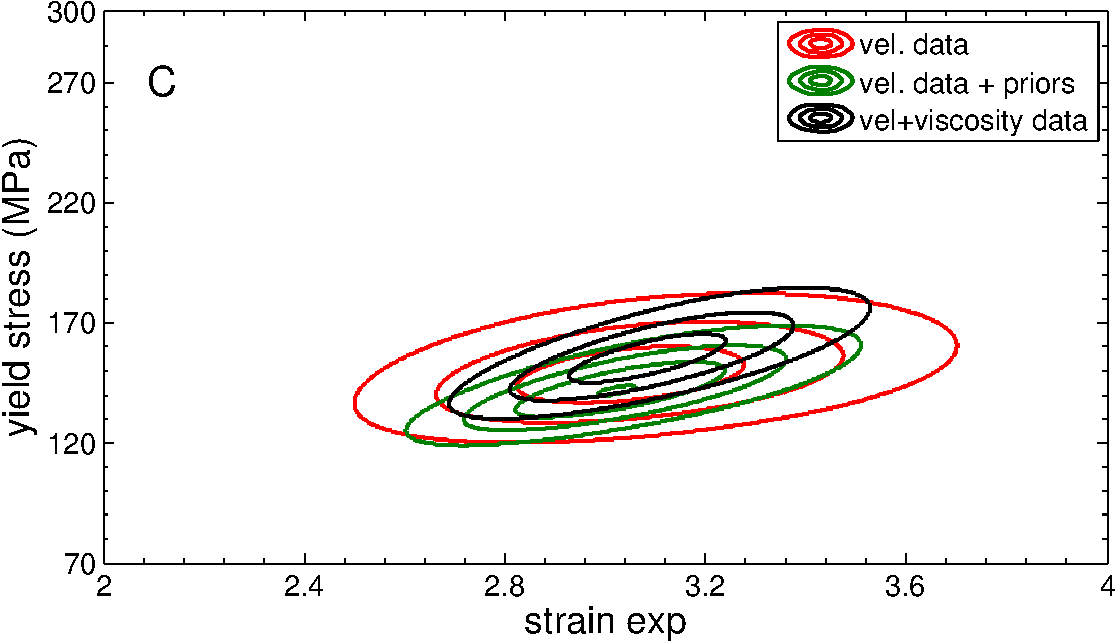
\includegraphics[height=35mm,width=52mm]{fig5c.pdf}%{mesh.pdf}
}
\subfigure[]{
\hspace{-0.8cm}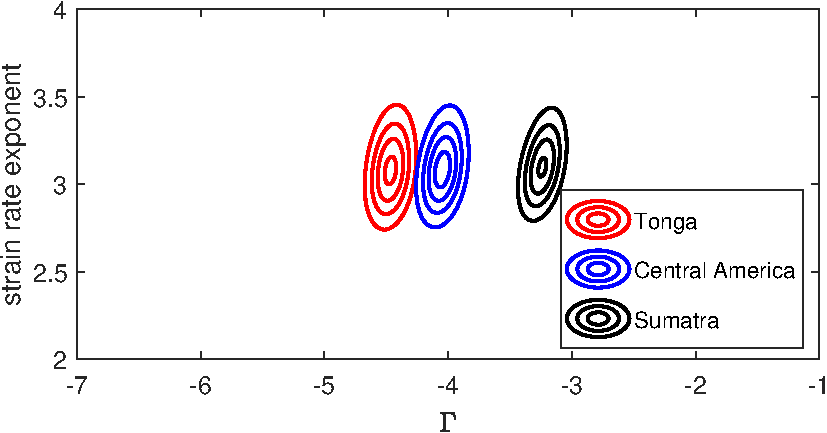
\includegraphics[height=35mm,width=52mm]{fig1new.pdf}%{mesh.pdf}
}
\subfigure[]{
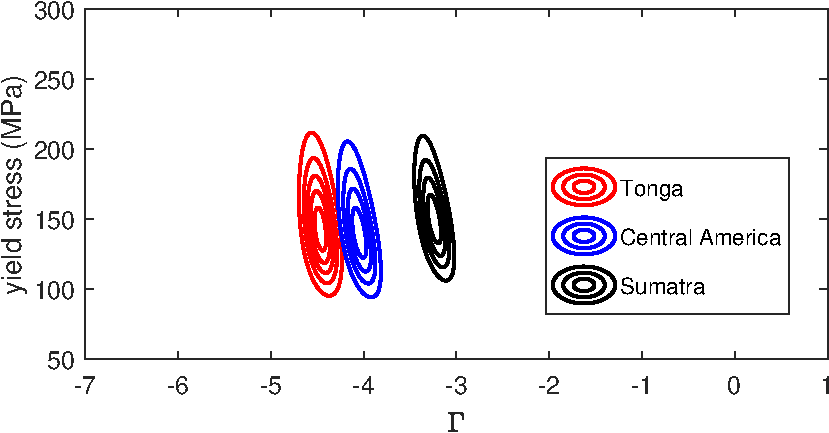
\includegraphics[height=35mm,width=52mm]{fig2new.pdf}%{mesh.pdf}
}
\hspace{0.1cm}\subfigure[]{
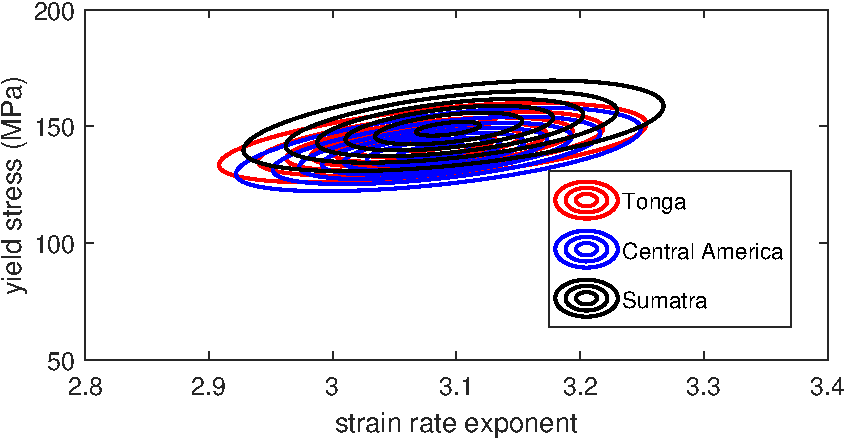
\includegraphics[height=35mm,width=52mm]{fig3new.pdf}%{mesh.pdf}
}
%\hspace{-0.2cm}\subfigure[]{
%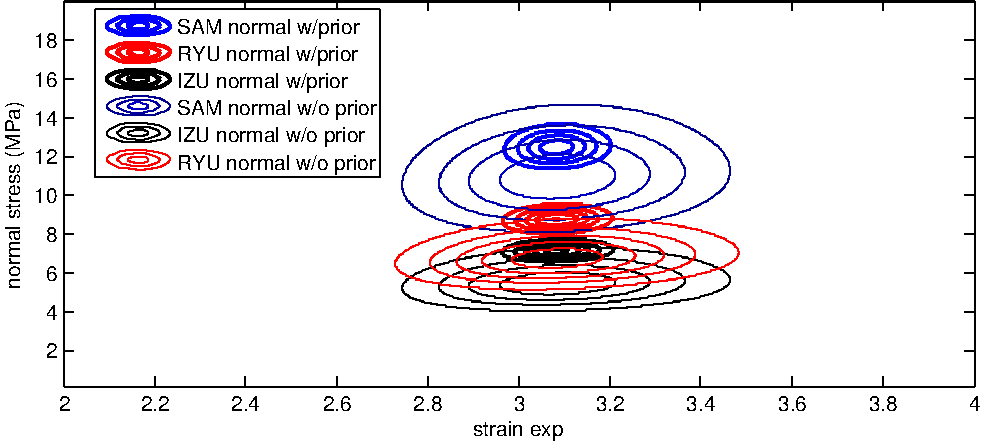
\includegraphics[height=35mm,width=58mm]{normal_comparison_prior2.pdf}%{mesh.pdf}
%}
%\hspace{-0.2cm}\subfigure[]{
%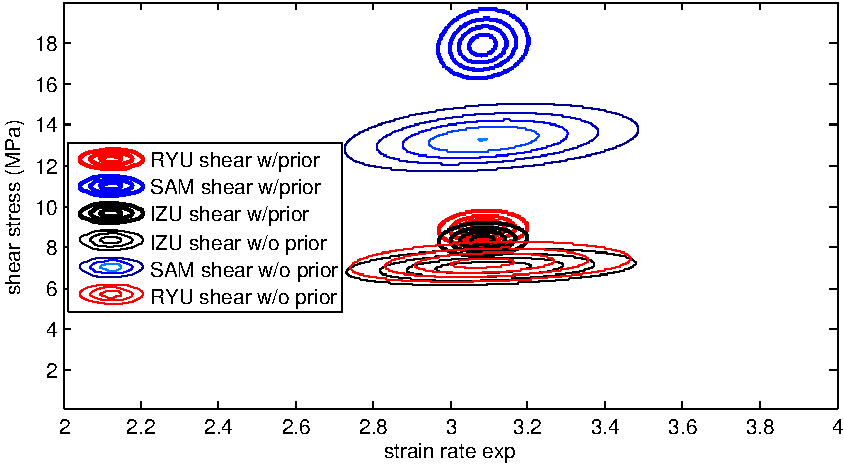
\includegraphics[height=35mm,width=58mm]{shear_comparison_prior.pdf}%{mesh.pdf}
%}
\caption{(A) Strain rate exponent vs. plate coupling. 
(B) Yield stress vs. plate coupling. 
(C) Yield stress vs. strain rate exponent for Case 1 (South America, Ryukyu and Izu-Bonin-(red: velocity constraint, black: velocity + viscosity constraints, blue: velocity constraint + priors) 
(D) Strain rate exponent vs. plate coupling. 
(E) Yield stress vs. plate coupling. 
(F) Yield stress vs. strain rate exponent  (Sumatra (red), Tonga (black) and Central America(blue))
\mgnote{Confusing Figure as colors mean different things in different panels. See me.}}
\label{fig:distrib}
\end{figure}

%An important idea is to know if these trade-offs exist for all inversions, that is with more (or less) inferred parameters, would these correlations remain the same. We find that these trade-offs are consistent when we reduce the parameter space in Case 2, i.e. marginalizing out the upper mantle prefactor, that this there still exists a negative correlation between yield stress and plate coupling in Case 2, which suggests that these rheological parameters are correlated in this way due to the underlying physics with respect to plate motions. Furthermore, we find that there is a positive correlation between the strain rate exponent and yield stress, implying that an increase in strain rate exponent (weakening of the upper mantle) precipitates an increase in yield stress (reduction in plate motion) to make plates resistant to bending.    

An open question about parameter trade-offs deals with additional data, more specifically the average effective viscosity in certain regions of the mantle. 
It is not apparent if these trade-offs will exist with additional data due to the different effects each parameter on both plate motions and average effective viscosity, even though we find similar values for the \textbf{MAP} point between the Case  (without effective viscosity data) and Case 3 (with effective viscosity data). In Fig.\ref{fig:distrib}c we see that the overall distributions are similar in that the trade-offs are the same; however, with the reduction in the variance for the strain rate exponent, the conditional distribution for the strain rate exponent and yield stress, when using average effective viscosity data, is smaller. This result supports the idea that the additional piece of effective viscosity data acts as prior information that can reduce the uncertainty of the inferred parameters. 
\mgnote{I think significantly, the slope of the yield stress vs. n increases when the viscosity data is included. Why is this the case? As I asked in the prior section, is the viscosity value that you constrain the system with, larger or smaller than the effective viscosity in the same region without such a constraint. Can you say, that the importance of the yield stress increases when you have added this additional constraint?}

\mgnote{We need to see the mean and variance of the Prior information on the plots because the reduction in the distribution in the Conditionals is not self evident}
While the correlations between the rheological parameters is important, using prior knowledge can further reduce the variance for the inferred rheological parameters. Using prior knowledge from laboratory experiments \citep{korenaga2008new}, we are able to reduce the variance of the plate couplings and global parameters in Case 4 as shown in Fig.\ref{fig:distrib}c, while retaining the same trade-offs between each rheological parameters, which is expected as we only reduced the acceptable range of the inferred parameters. While the conditional distributions for the larger cross-section show that there is indeed trade-offs in plate couplings and global parameters, is is unknown if these trade-offs exist for all subduction zones. To this end, we compared the conditional distributions for Sumatra, Tonga and Central America in Fig.\ref{fig:distrib}d,e and f. 


In Fig.\ref{fig:distrib}d-e, we find similar trade-offs between the plate coupling and strain rate exponent, that is an increase in plate coupling (an increase in viscosity within the fault zone) would lead to an increase in the strain rate exponent (by promoting more shear thinning) so as to increase plate motion. Similarly, as the plate coupling increases, the yield stress decreases (by promoting more dynamic weakening) so that plates can overcome the resistance from an increase in plate coupling. Furthermore, the same trade-off (positive correlation) between the strain rate exponent and yield stress is found for the Sumatra, Tonga and Central America (Fig.\ref{fig:distrib}f). 

\mgnote{Let's Discuss. Is there a conditional distribution that does along with this (or these) inversions? Case numbers's?}
We can visually see these trade-offs in the conditional distributions from the effective viscosity in Fig.\ref{fig:visc_smaller} for Sumatra and Central America. We see that there is sufficient strain rate weakening in the upper mantle for each model for both Sumatra and Central America, however, the amount of yielding from dynamic weakening changes in the hinge zone and overriding plate between Sumatra and Central America. We find in Fig.\ref{fig:visc_smaller} that there is a larger plate coupling for Sumatra relative to Central America, which  yields more dynamic weakening in the overriding plate (more strain). When comparing the effective viscosity of the slabs for Sumatra and Central America, we find that the final viscosity structure suggests that the Central America slab is stronger due to less dynamic weakening and more decoupling between the overriding and subducting plate. 



\begin{figure}[H]
\centering

\hspace{-1.0cm}\subfigure{
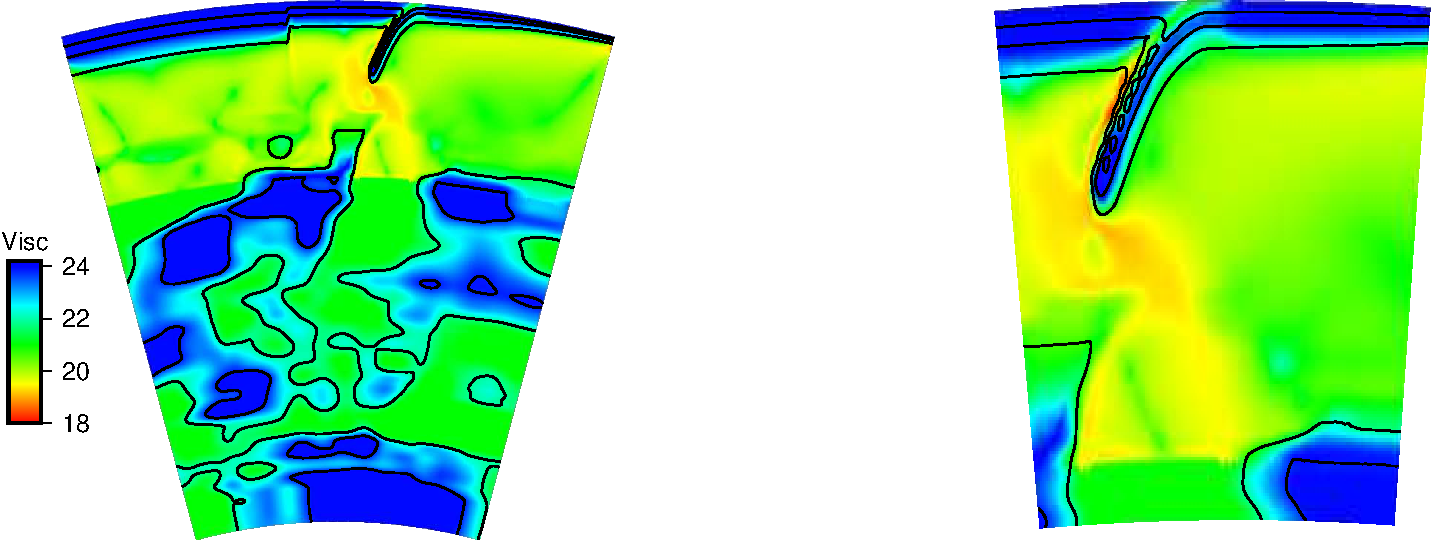
\includegraphics[scale =0.5]{contour_theory.pdf}%{mesh.pdf}
}

\hspace{0.2cm}\subfigure{
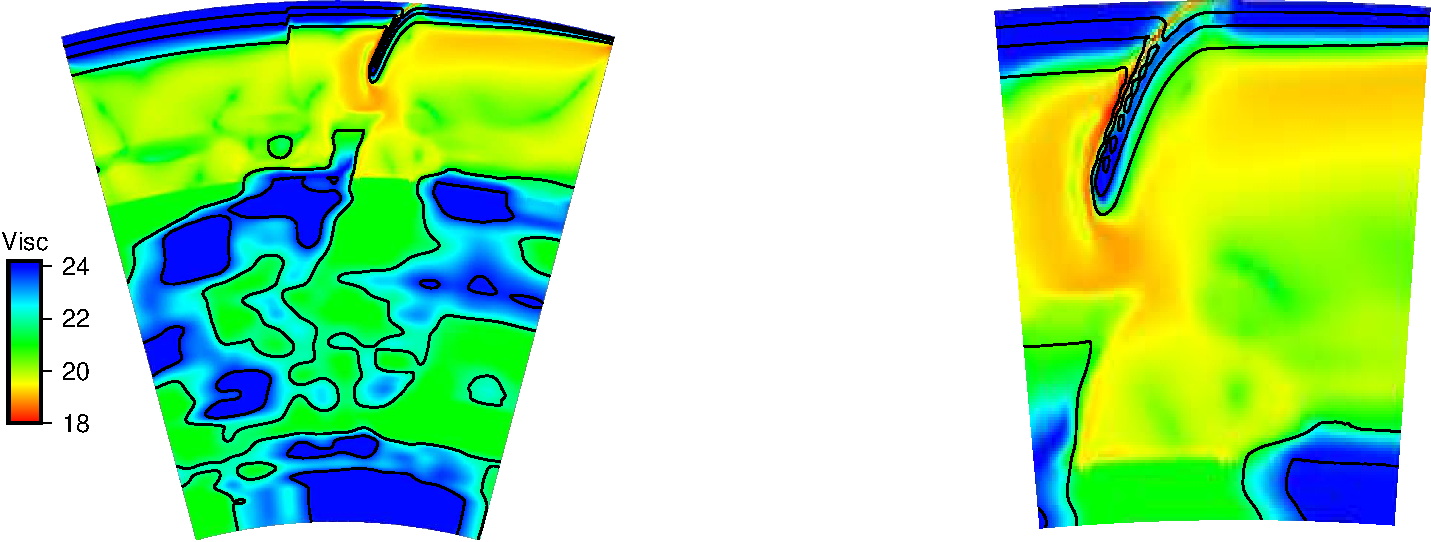
\includegraphics[scale=0.5]{contour_theory2.pdf}%{mesh.pdf}
}
%\hspace{-0.2cm}\subfigure[]{
%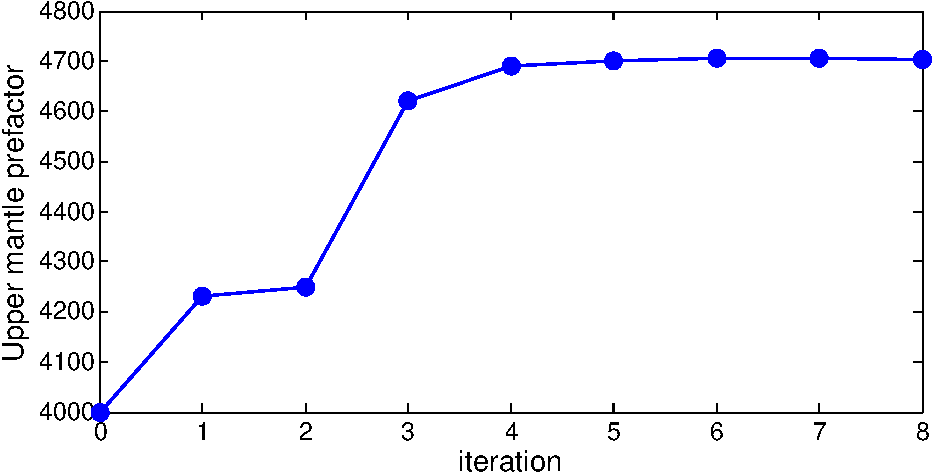
\includegraphics[height=35mm,width=58mm]{um_chap4.pdf}%{mesh.pdf}
%}
\caption{\mgnote{Case numbers's? Are these different iterations for a single inversion} Effective viscosity for a forward model for Middle America (A) Coupled ($\Gamma = 4.0 \cdot 10^{-3}$, $\sigma_y = 160$ MPa, and $n = 3.08$) (B) Zoom in of Middle America and increase in strain rate exponent (C) ($\Gamma = 1.0 \cdot 10^{-5}$, $\sigma_y = 160$ MPa, $n = 3.08$)
(B) Zoom in of Central America subduction zone. \mgnote{You need to consistenly use Middle versus Central America.}}
\label{fig:middle_physics}
\end{figure}

\mgnote{Are these different iterations or different Case numbers's?}To further elucidate these trade-offs, we consider a \mgnote{This is not a thought experiment } thought-experiment where we consider two forward models of Middle America in (Fig.\ref{fig:middle_physics}a). In this example, we consider a coupled Central America subduction zone in Fig.\ref{fig:middle_physics}a, and see  that for a larger coupling the slab would then slow down and the amount of weakening around the slab decreases, resulting in an increase in viscosity around the slab. However, when the coupling is decreased ($\Gamma=4\cdot 10^{-5}$), the amount of strain strain rate weakening increases as does the velocity of the plate. This interplay between the rheological parameters is important as it demonstrates a strong interaction between the global rheological parameters (yield stress and strain rate exponent) and local coupling parameter.



\begin{figure}[H]
\centering
\hspace{-0.85cm}\subfigure{
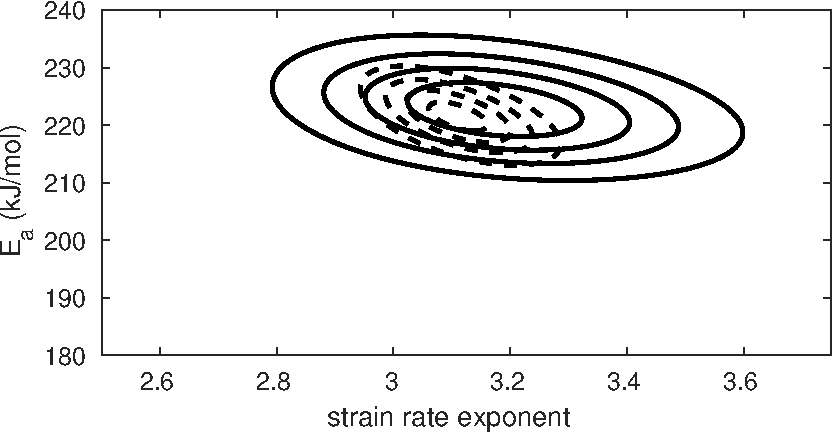
\includegraphics[height=35mm,width=52mm]{ea_strain_large.pdf}%{mesh.pdf}
}
\hspace{-0.1cm}\subfigure{
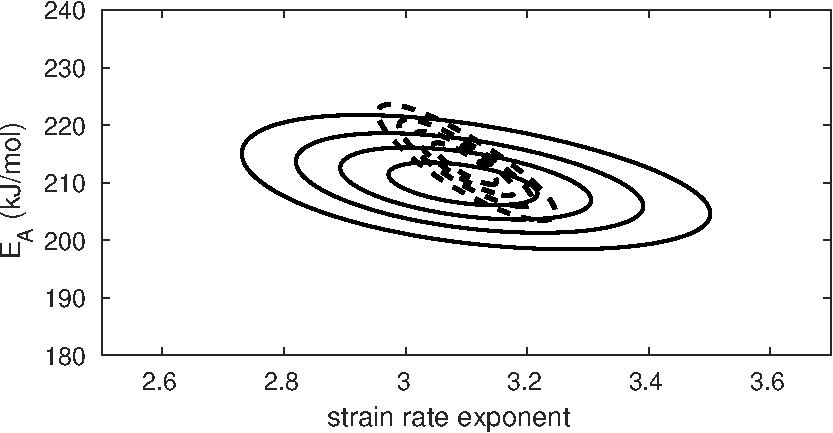
\includegraphics[height=35mm,width=52mm]{ea_strain_sumatra.pdf}%{mesh.pdf}
}
\hspace{-0.1cm}\subfigure{
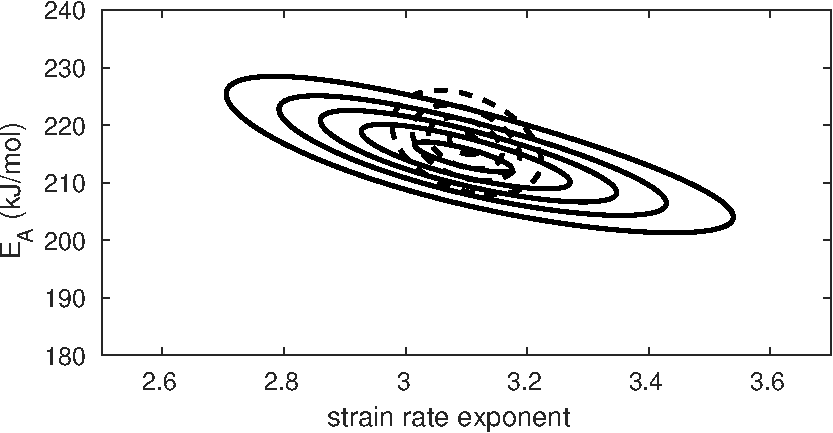
\includegraphics[height=35mm,width=52mm]{ea_strain_central.pdf}%{mesh.pdf}
}
 

\caption{Activation energy vs. strain rate exponent for (A)Sumatra. 
(B) Central America. 
(C) Tonga (Dashed lines include priors) }
\label{fig:activ_distrib}
\end{figure}


One of the key analyses that was developed in this chapter was the characterization of the uncertainty of the stresses (shear and normal) of each plate boundary that is built upon a Gaussian approximation around the \textbf{MAP} point for each inversion. We apply this approach to our models as shown in Fig.\ref{fig:shear_smaller}a,b, where we compare the mean normal and shear stresses of each plate boundary and find that there is a similar pattern of the partitioning between the least coupled subduction zones of Ryukyu and Izu-Bonin to the more coupled subduction zone of South America. Similar to Fig.\ref{fig:distrib}, the same pattern of a more coupled South America plate boundary appears (both normal and shear stresses), regardless of the global parameter. However, we note that the mean of the computed normal stress is lower than the shear stresses, which is certainly not expected.



\begin{figure}[H]
\centering
\hspace{-0.85cm}\subfigure{
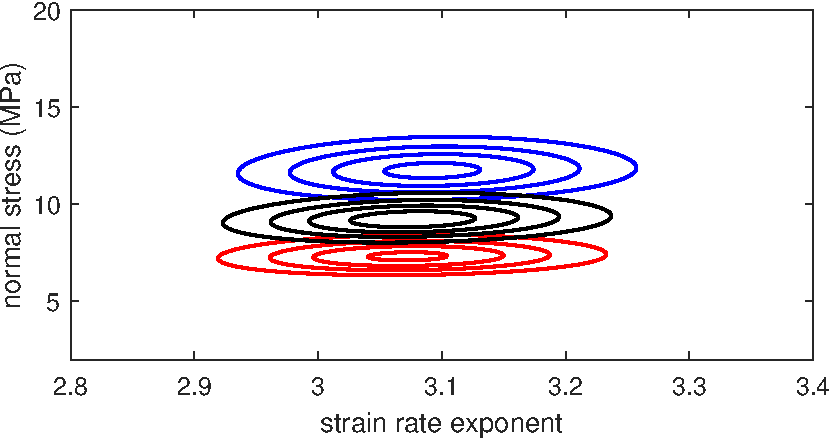
\includegraphics[height=35mm,width=52mm]{fig8new.pdf}%{mesh.pdf}
}
\hspace{-0.1cm}\subfigure{
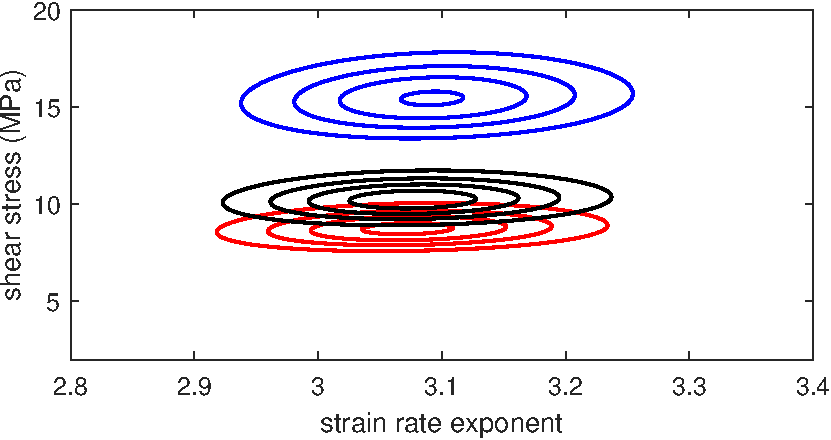
\includegraphics[height=35mm,width=52mm]{fig9new.pdf}%{mesh.pdf}
}

\caption{(A)Normal Stress vs. strain rate exponent. 
(B) Shear stress vs. strain rate exponent. 
 for WEP}
\label{fig:stress_distrib1}
\end{figure}


\begin{figure}[H]
\centering
\hspace{-0.2cm}\subfigure[]{
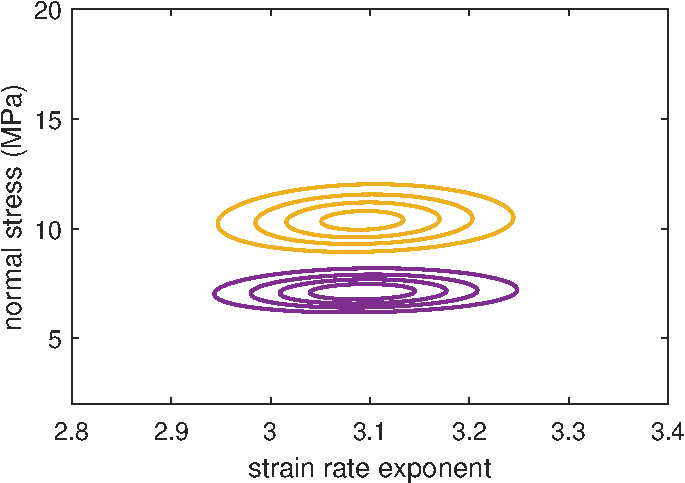
\includegraphics[height=35mm,width=58mm]{fig3.pdf}%{mesh.pdf}
}
\hspace{-0.2cm}\subfigure[]{
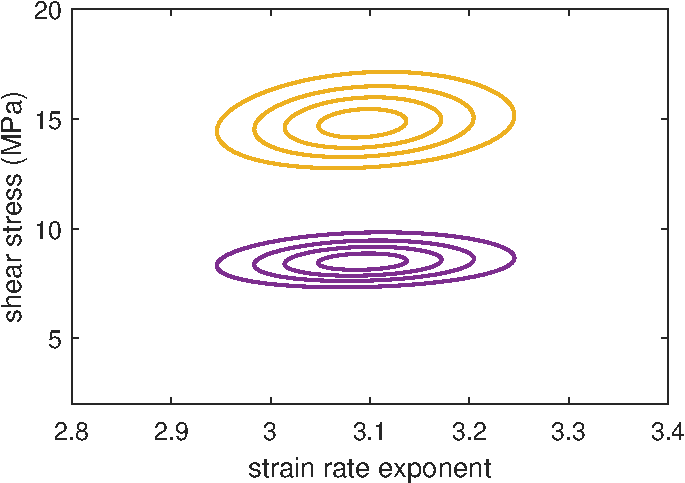
\includegraphics[height=35mm,width=58mm]{fig4.pdf}%{mesh.pdf}
}
\hspace{-0.2cm}\subfigure[normal stresses]{
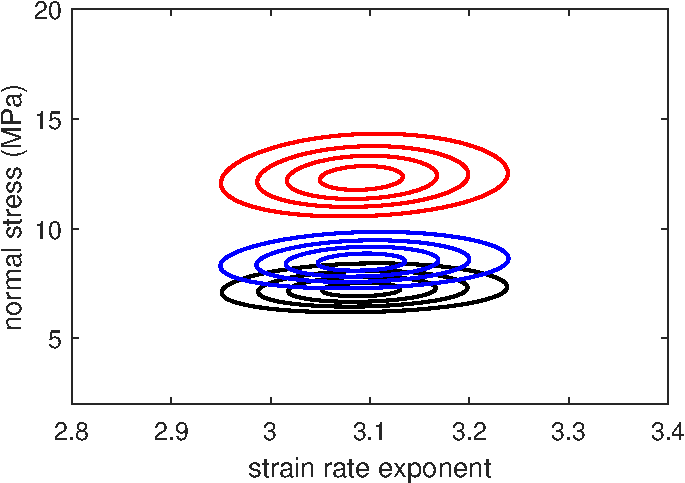
\includegraphics[height=35mm,width=58mm]{fig5.pdf}%{mesh.pdf}
}
\hspace{-0.2cm}\subfigure[shear stresses]{
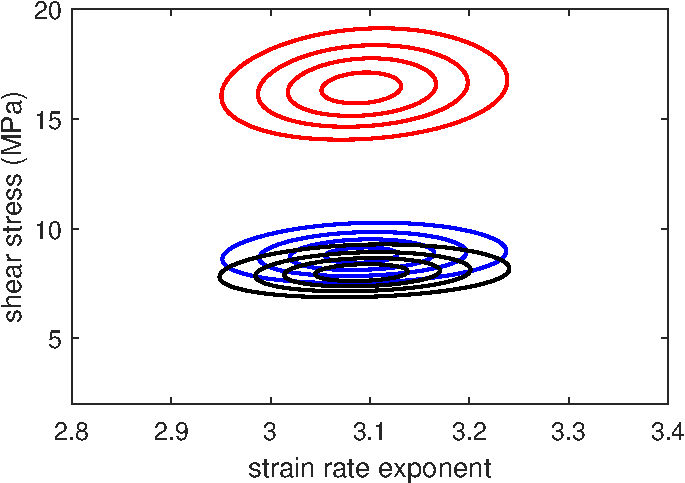
\includegraphics[height=35mm,width=58mm]{fig6.pdf}%{mesh.pdf}
}
\caption{
\mgnote{In A and B there is a 'dashed' line in the label box but no such line in the figures.}
(A) Normal stress comparison and 
(B) shear stress comparison for Tonga cross section (Yellow contours are for South America while purple contours are for Tonga). 
(C) Normal stress comparison and (D) shear stress comparison for Tonga and South America\mgnote{Different colors are needed in C and D than used in A and B.}}
\label{fig:shear_smaller}
\end{figure}


We similarly compared the stress conditional distributions for Sumatra and Tonga in Fig.\ref{fig:shear_smaller}c,d and find that the shear average shear stress in the fault zones are larger than the normal stress. Similar to South America, we find that there is a partitioning of subudction zones for both shear and normal stresses, where Sumatra is more coupled than Tonga.


\begin{figure}[H]
\centering
\hspace{-0.2cm}\subfigure[]{
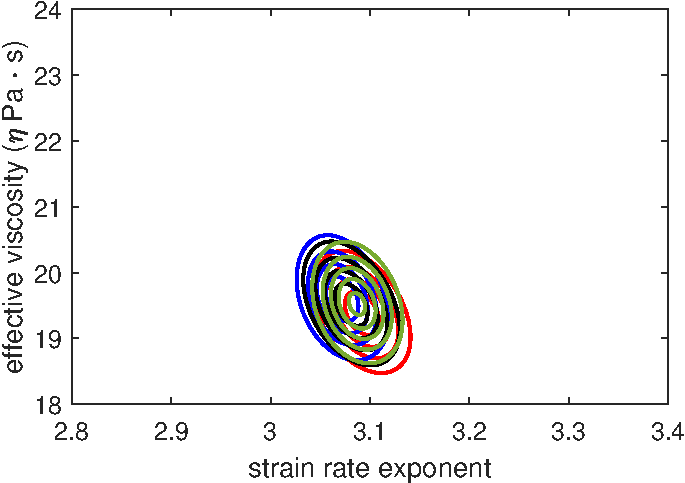
\includegraphics[height=35mm,width=58mm]{fig7.pdf}%{mesh.pdf}
}
\hspace{-0.2cm}\subfigure[]{
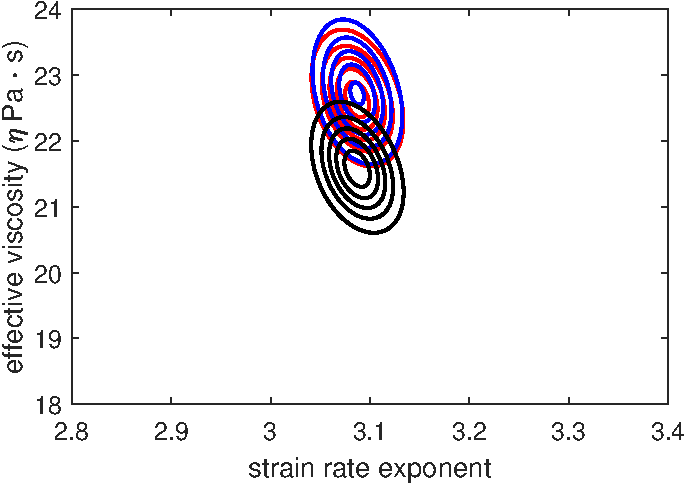
\includegraphics[height=35mm,width=58mm]{fig8.pdf}%{mesh.pdf}
}
\hspace{-0.2cm}\subfigure[normal stresses]{
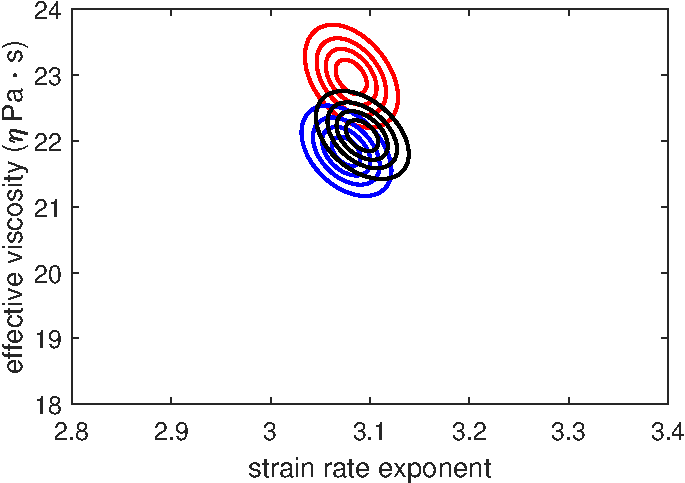
\includegraphics[height=35mm,width=58mm]{fig9.pdf}%{mesh.pdf}
}
\hspace{-0.2cm}\subfigure[shear stresses]{
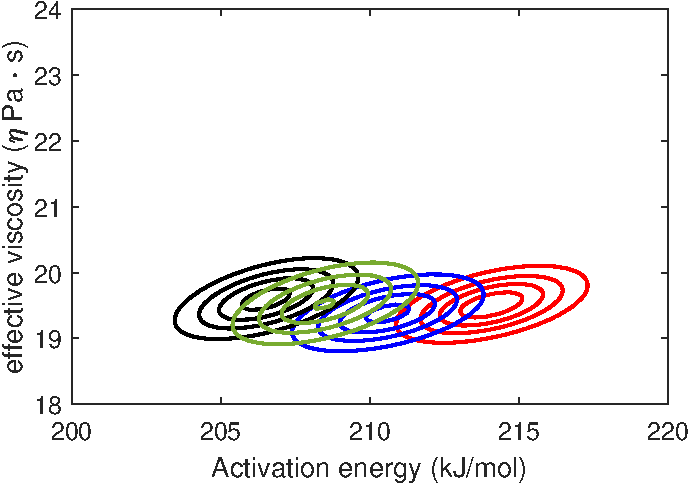
\includegraphics[height=35mm,width=58mm]{fig10.pdf}%{mesh.pdf}
}
\caption{
\mgnote{In A and B there is a 'dashed' line in the label box but no such line in the figures.}
(A) Average Effective Viscosity vs. strain rate exponent in the upper mantle  
(B)  Average Effective Viscosity vs. strain rate exponent in the hinge zones  for Sumatra, Central America and Tonga
(C) Average Effective Viscosity vs. strain rate exponent for WEP (D) Average Effective Viscosity vs. Activation energy for WEP, Sumatra, Central America and Tonga}
\label{fig:shear_smaller}
\end{figure}

\section{Discussion}
In our studies, we build upon the work done in \citep{ratnaswamy2015adjoint} in multiple ways: (1)adding additional observations (effective viscosity) (2)using realistic temperature data and fault zone structures (3)plate motion data from MORVEL56 and (4)covariance estimates on quantities of interest (QOI) that are not inferred such as stresses and average effective viscosities (extrinsic parameters). When incorporating these methods into this optimization framework, we are able to analyze the relationships between the rheological (intrinsic) properties vs extrinsic quantities as well as any improvements in the uncertainty we get from adding additional data.

 We considered four crosses sections: (1)WEP (2)Sumatra (3)Tonga and (4) Central America as they represent varying spectrum of the seismic coupling and therefore inferring the rheological parameters for each of these cross-sections can tell us to what degree the inferred parameters vary for each subduction zone. The WEP model contains three subduction zones:(1)South America (2)Izu-Bonin and (3)Ryukyu, where the South America subduction zone is thought to be the most seismically coupled while Izu-Bonin and Ryukyu are thought of as the least seismically coupled \citep{scholz2012seismic}. With the WEP model, we found that the strain rate exponent across all models is slightly larger than 3.0 (Cases ). Even without prior knowledge, the likelihood distribution suggests that a \textbf{MAP} point of 3.072 in Case is sufficient to predict observed plate motions. 
  
  The strain rate value of 3.0 is similar with those that obtained from experiments, though those experiments are larger (approximately 3.5). The larger strain rate exponent from from experiments can be due to uncertainty in both the conditions such as pressure and temperature. Furthermore, we find in the Sumatra, Central America and Tonga cases that we infer a strain rate exponent between 3.076-3.12, which is in the range of those obtained in Case for WEP. Therefore, there seems to be a relationship between these 2D models that regardless of the cross-section, the preferred strain rate exponent in the upper mantle should be larger than 3.0. Furthermore, the strain rate we obtain in all of our inversions also show a weak asthenosphere, (approximately $10^{19-20}Pa\cdot s$), which is similarly found in other studies that have tried to constrain the average effective viscosity. An important caveat is that while the nonlinear strain rate exponent is important for weakening in the upper mantle, it is not the only physical process as we do not account for water weakening.
  
  The yield stress is an important quantity as it locally controls weakening in the slabs. However, our yield stress is not the same as the Byerlee law since our yield stress is a global quantity (not depth-dependent). We typically find yield stresses that are approximately $150 \space MPa$ in our inferences for the WEP cross-section. While the 150 MPa value is global for this cross-section it does not have the same effect for each subduction zone, that is there is a different amount of dynamic weakening in each of the slabs. We find in Fig., that there is more dynamic weakening in the hinge zone for the Nazca plate compared to Ryukyu and the Pacific plate. This dynamic weakening is a product of both the plate coupling and the yield stress. We note that this yield stress is larger than those from estimates in seismicity, as it is assumed that the yield stress should be less than $10 \space MPa$. However, by the very nature our models only can inform how strong slabs because we do not allow for yielding in the fault zones.
  
  Therefore, a large yield stress value such as $132 MPa$ suggests that slabs are sufficiently strong such that they can accommodate large stress values which is not a surprise as it has been thought that slabs are strong enough to be stress guides \citep{Stadler27082010}. In Case , the yield stress of 150 MPa suggests that slabs need to not only have a larger viscosity contrast but need to have a certain stress threshold to propagate stresses from the mantle to the plates. An important question is how large of a viscosity contrast relates to the stresses within slabs. Within our forward models, we apriori bound the effective viscosity by $\mathcal{O}(6)$ magnitudes, where the majority of the viscosity variations occur between the slab and the weak-zone. Therefore, the relationship between the effective viscosity and stress within slabs is best understood from the point of view of the viscosity variations between the asthenosphere and slab. In our models, the average effective viscosity within the slab is approximately $10^{24}\space Pa\cdot s$, while the average effective viscosity in the asthenosphere is $3\cdot 10^{20}\space Pa\cdot s$, or approximately $\mathcal{O}(4)$ magnitude in viscosity variations. Therefore, there seems to be a minimum value of variations in viscosity for slabs to act as stress guides.   We also find that there is a variation in the dynamic weakening for Sumatra, Central America and Tonga subduction zones. While the inferred yield stresses for each of those models vary between 135-147 MPa, they still exhibit different amounts of weakening in the hinge zone, where there is more of a reduction of the effective viscosity for Sumatra compared to Tonga and Central America.
  
  The activation energy is an important quantity that we added to our parameter inferences for each of the cross-sections. We find that the inferred activation energy is approximately 215 kJ/mol for the WEP cross-section in Case . Similarly, we note that in the smaller cross-sections in Sumatra, that the activation energy is 219 kJ/mol. We find that this value provides sufficiently strong plates and slabs while providing a strong contrast between the effective viscosity of the upper mantle and the plates. As mentioned earlier, there is a relationship between the amount of dynamic weakening in the hinge zone based on the amount of coupling and the yield stress. Looking at the WEP cross-section, we find that for all the cases () there is a partitioning of the weakfactors for each subduction zone. In each case, we find that there is at least an order of magnitude of increase in the South America subduction zone weakfactor compared to Ryukyu and Izu-Bonin. Furthermore, the weakfactor for Ryukyu is similar to Izu-Bonin, with Ryukyu's weakfactor being slightly larger than Izu-Bonin. Furthermore, we find that with this increased weakfactor for South America, there is more dynamic weakening in the more coupled South America subduction zone so as to 
  
  An important recurring result within our inversions is the trade-offs between the rheological parameters such as the strain rate exponent and yield stress. To review, the weakfactor controls the amount of resistance along the plate-boundary  interface, the strain rate exponent controls the amount of shear-thinning, while the yield stress controls the amount of weakening within plates and slabs. In each of the cross-sections (WEP, Sumatra, Tonga and Central America) we find that there is a negative correlation between the strain rate exponent and the yield stress, which was similarly found in \citep{ratnaswamy2015adjoint}. This result is significant as it suggests that the even with the MORVEL56-NNR plate motion model, there still is a preferred correlation between the strain rate exponent and yield stress that was similarly found for synthetic models in \citep{ratnaswamy2015adjoint}. Further examining the negative correlation between the strain rate exponent and yield stress, when there is significant yielding in hinge zone as in WEP (Fig.), the reduction effective viscosity causes the slab to fall into the upper mantle, which increases the strain rate and effectively increases plate speed due to the reduced bending force. Therefore, to compensate for this increase in plate motion either the strain rate exponent or weakfactor must change.
  
  The correlation between the weakfactor and yield stress is an emergent trade-off we see within all the cross-section models. We find that as the weakfactor increases (channel in the fault zone becomes more viscous), there is a negative correlation between the yield stress. This negative correlation implies that when the weakfactor increases, there is a reduction in the yield stress which promotes weakening in the hinge zone to counter the increased resistance. In particular, we see that as yielding occurs as plates bend in the Nazca plate in WEP, we find that the weakfactor is comparably larger than Ryukyu and Izu-Bonin (where both of those subduction zones have less yielding). Similarly, this trade-off occurs in the Sumatra model, where we see that there is a significant amount of coupling while there is sufficient yielding within the slab. This trade-off between the weakfactor and yield stress comes about because the increased resistance from the plate coupling causes more weakening around the slab to allow for it to fall into the upper mantle.  The Middle America cross-section represents the opposite case compared to Sumatra, that is, there is a decoupling between the overriding plate and subduction zone. This decoupling represents an increase in plate speeed, therefore to compensate for the increase in plate velocity would require an increase in the bending force in the hinge zone-that is there would be an increase in the yield stress to increase the bending force.
  
   While the tradeoff between the weakfactor and yield stress is demonstrated for WEP and the smaller cross-section models, there seems to be a correlation between the intrinsic mechanical coupling (weakfactor) and the seismic coupling in Table \ref{table:parameters}. Notably, there is a delineation of subduction zones between those that are mechanically coupled. In all of our WEP models, we find that the South America subduction zone is the most (mechanically) coupled compared to Ryukyu regardless of which parameter we held fixed. This mechanical coupling between South America seems to be correlated to the seismically coupled values from Chile in Table \ref{table:parameters}. The other end of the spectrum is where there is the relationship between the mechanical coupling and seismic coupling. We find that for the Sumatra cross-section, there is a larger mechanical coupling than Central America.
   
   \begin{table}[H]
  \caption{Summary of seismic coupling coefficients ($\chi_s$) is the seismic coupling coefficient, while $\chi_g$ is the geodetic coupling coefficient \citep{scholz2012seismic}.} % title of Table
  \centering  % used for centering table
  \begin{tabular}{c c c c c c} % centered columns (2 columns)
    \hline \hline                        %inserts double horizontal lines
    Subduction Zone & $\chi_s$ & $\chi_g$ & $\sigma_n (MPa)$ & $\sigma_t (MPa)$ & $\Gamma$ \\ [0.5ex] % inserts table
    %heading
    \hline                  % inserts single horizontal line
    Izu-Bonin &0.01 &N/A &7.22 &7.99 & $7.42 \cdot 10^{-6}$\\
    South Ryukyu  &0.05 &N/A &8.47&8.72 & $9.11 \cdot 10^{-6}$\\
    Central Chile &0.70 &1.0 &12.3 &16.4 & $7.02 \cdot 10^{-4}$ \\
    Sumatra &0.5-0.83 &1.0 &11.73 & 15.33 &$3.93 \cdot 10^{-4}$\\
    Central America &0.10 &0.20 &9.22 & 10.23 & $5.51 \cdot 10^{-5}$ \\
    North$/$South Tonga & $0.66/0.14$ &N/A &7.32 & 8.74 & $8.32 \cdot 10^{-5}$ \\
    \hline %inserts single line
  \end{tabular}
  \label{table:coupling_summary} % is used to refer this table in the text
\end{table}

   
   While we are able to estimate the mechanical coupling between subduction zones, we need to look at the stresses within the subduction zones to compare to those provided by seismological constraints. We find that in all of our cases (WEP, Sumatra, Central America and Tonga) that the estimates of shear and normal stresses are less than 20 MPa, which satisfies seismological constraints, suggesting that the inferred rheological parameters give rise a reasonable state of stress. While the stress values are in the correct range, we find that the conditional distributions have bounds on how large the stresses are-which are under 20 MPa. Examining the stress conditionals for WEP, we find that the \textbf{MAP} point for the shear stresses are consistently larger than those of the normal stresses-which suggests a problem as fault zones since the normal stress should be larger than then shear stress ($\textbf{F}_s = \mu\textbf{F}_m$). However, we do not use a an elasticity or plasticity law within the fault zones-that is it is a purely viscous flow. This flow can be thought of as Couette flow as the viscous weak channel has the slab moving above the weak viscous layer.
   
   Ultimately, these \textbf{MAP} point values are within range of values that are acceptable; however, we need to take into account these viscous stress values are related to seismic couplings. A subduction zone that is very coupled has a seismic coupling close to 1.0., while those that are least seismically coupled have values closer to 0.  In Table \ref{table:parameters}, we see that the seismic and geodetic coupling ($\chi_s$ and $\chi_g$) for Peru (Central and South), while Chile and Sumatra have larger geodetic couplings that are large, while Tonga has a seismic coupling that is less than 1 in Table \ref{table:parameters}. We find a similar ordering compared to that obtained from seismic coupling, in that the largest shear stresses belong to the South America, Sumatra plate boundaries compared to Izu-Bonin, Ryukyu and Tonga-which suggests that there is a correlation between mechanical and seismic coupling. However, to truly test if this relationship holds, similar parameter inferences need to be made on 3D models where there is both toroidal and poloidal flow. Furthermore, extensions of this work should seek to include plasticity within the fault zones for a better estimate of the shear and normal stresses there; however, with plasticity included, there are additional parameters such as the cohesion that needs to be accounted for. In these studies, we have laid the foundation for using multiple pieces of data to better constrain the strain rate exponent. Furthermore, we extended our formulation to forward predict the uncertainty in the extrinsic quantities by generating a Gaussian approximation to the shear and normal stresses. Those approximations for the stresses show that there is a partitioning of seismically coupled subduction zones in the mechanical sense, which suggests that regardless of what the strain rate exponent and  yield stress, there is a preferred mechanical coupling of subduction zones. To verify this result, it needs to be tested out with global models.
                 








\appendix
\section{Derived Covariance Estimates}
We have previously set models in how to estimate quantities that are are inferred such as the stresses. In this section, we will thoroughly discuss how to apply this Gaussian approximation to various quantities of interest. Mapping of covariance matrices from one space to another requires  a transformation,i.e. using the Jacobian. As an example, we will look at transforming a Gaussian distribution for the inferred yield stress and strain rate exponent, that is $\ppi(\mm):= \mathcal{N}([n,\ssigma_y],\mathcal C) \rightarrow \ssigma(\gamma \mm)$, where we look at the scaled space between the parameters. To determine the mapping of the covariance we make use of,
\underline{Case 1: 1D Normal}
\begin{equation}
\frac{\partial \ssigma}{\partial \mm} = \gamma
\end{equation}
leading to
\begin{equation}
\ppi_2 = \mathcal N(\mu,\gamma^2\sigma)
\end{equation}
\underline{Case 2: 2D Normal}
We consider the case when we apply a stretch factor in the form of $\gamma = [\gamma_1, \gamma_2]$, that is $\mm = [\mm_1, \mm_2]$. Therefore $\ssigma = [\gamma_1 \mm_1, \gamma_2 \mm_2]$. The follwoing now holds
\begin{equation}
\frac{\partial \ssigma}{\partial \mm} = 
\begin{bmatrix}
\gamma_1 & 0 \\
0 & \gamma_2 \\
\end{bmatrix}
\end{equation}
leading to
\begin{equation}
\mathcal C = 
\begin{bmatrix}
\gamma_1^2 a & \gamma_1 \gamma_2 b \\
\gamma_1 \gamma_2 b & \gamma_2^2 c \\
\end{bmatrix}
\end{equation}

\begin{equation}
\ppi_2 = \mathcal N(\mu,\gamma^2\sigma)
\end{equation}
An important point is to construct the covariance matrix for the relationship between the stress and inferred parameters (strain rate exponent, yield stress). To do so, we form the vector $\ssigma_{a}$ such that  $\ssigma_a = (\ssigma, n,\sigma_y..)^T$. Doing so, we find the Jacobian is
\begin{equation}
\frac{\partial \ssigma_a}{\partial \mm} = \frac{\partial [\ssigma, n, \sigma_y...]^T}{\partial \mm}
\end{equation}
which results in 
\begin{equation}
\mathcal C = 
\begin{bmatrix}
\frac{\partial \ssigma}{\partial n} & \frac{\partial \ssigma_{a}}{\partial \sigma_y} \\
\frac{\partial n}{\partial n}& \frac{\partial n}{\partial \sigma_y} \\
\frac{\partial \sigma_y}{\partial n}& \frac{\partial \sigma_y}{\partial \sigma_y} \\
\end{bmatrix}
\end{equation}
which leads to 
\begin{equation}
\mathcal C = 
\begin{bmatrix}
\frac{\partial \ssigma}{\partial n} & \frac{\partial \ssigma_{a}}{\partial \sigma_y} \\
1 & 0\\
0 & 1 \\
\end{bmatrix}
\end{equation}

\begin{figure}[H]
\centering
\hspace{-1.2cm}\subfigure{
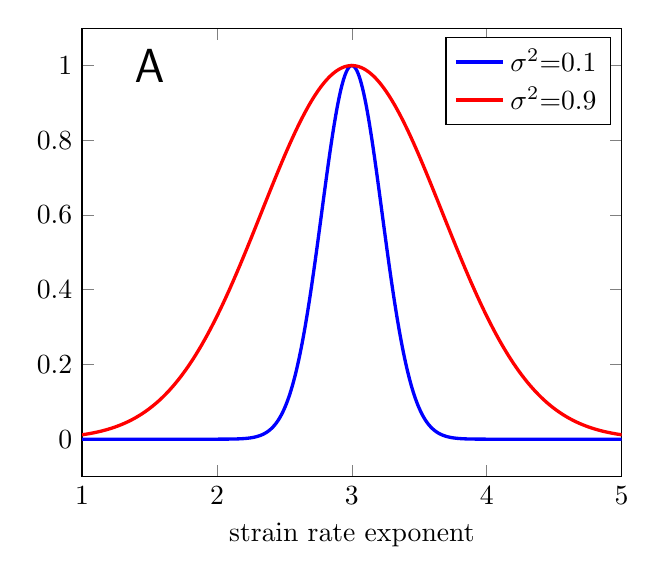
\begin{tikzpicture} 
\begin{axis}[ xlabel=strain rate exponent,xmin=1.0, xmax=5.0 ] % invoke external gnuplot as % calculator: 
  \addplot [mark=none,very thick, blue, samples=1000]{exp(-(x-3.0)^2/0.1)}; 
  \addlegendentry{$\sigma^2$=0.1}
  \addplot [mark=none,very thick, red, samples=1000]{exp(-(x-3.0)^2/0.9)}; 
  \addlegendentry{$\sigma^2$=0.9}
\node[font=\fontsize{18}{18}\sffamily] at (axis cs:1.5,1.0){A};


\end{axis} 
\end{tikzpicture}
}
\end{figure}
\subsection*{Uncertainty estimates for Effective viscosity}
While we have developed this machinery for normal and shear stresses, we can extend it to the effective viscosity in a region. The average effective effective viscosity we are interested in is,
\begin{equation}
 \eta_{avg} = \exp(\int_{\Omega_i} \log \eta d\Omega_i)
 \end{equation}
The jacobian is then,
\begin{equation}
\frac{\partial \eta_{avg}}{\partial \mm} = \eta_{avg}\int_{\Omega_i} \frac{\eta){,i}}{\eta}
\end{equation}
The transformation then yields 
\begin{equation}
\mathcal C = 
\begin{bmatrix}
\frac{\partial \ssigma}{\partial n} & \dots & \frac{\partial \ssigma_{a}}{\partial \sigma_y} \\
1 &  0 & \dots & 0\\
0 & 1 & \dots & 0 \\
\vdots & \vdots & \ddots  & 0 \\
0 &0 & \dots & 1 

\end{bmatrix}
\end{equation}
%\section*{Conclusion}

\bibliography{references}


\end{document}
